\documentclass[a4paper, 10pt, twoside]{article}

\usepackage[top=1in, bottom=1in, left=1in, right=1in]{geometry}
\usepackage[utf8]{inputenc}
\usepackage[spanish, es-ucroman, es-noquoting, activeacute]{babel}
\usepackage{setspace}
\usepackage{fancyhdr}
\usepackage{lastpage}
\usepackage{amsmath}
\usepackage{amsfonts}
\usepackage{amsthm}
\usepackage{algpseudocode}
\usepackage[]{algorithm2e}
\usepackage{verbatim}
\usepackage{fancyvrb}
\usepackage{graphicx}
\usepackage{float}
\usepackage{enumitem} % Provee macro \setlist
\usepackage{tabularx}
\usepackage{multirow}
\usepackage{hyperref}
\usepackage{lscape}
\usepackage{xspace}
\usepackage{qtree}
\usepackage{color}
\usepackage[toc, page]{appendix}


% Codigo fuente.
\usepackage{listings}
\lstset{
  language=C++,
  basicstyle=\small\sffamily,
  numbers=left,
  numberstyle=\tiny,
  frame=tb,
  columns=fullflexible,
  showstringspaces=false
}

\newcommand\todo[1]{\Large\textbf{\text{?}color{red}{#1}}\normalsize}


\usepackage{chngcntr} % Numeracion granular de distintos entornos.
\counterwithin{table}{section}
\AtBeginDocument{\counterwithin{lstlisting}{section}}



%%%%%%%%%% Constantes - Inicio %%%%%%%%%%
\newcommand{\titulo}{Trabajo Práctico 1}
\newcommand{\materia}{Redes Neuronales}
\newcommand{\integrantes}{Barijhoff - Ishikame - Russo}
\newcommand{\cuatrimestre}{Segundo Cuatrimestre de 2016}
%%%%%%%%%% Constantes - Fin %%%%%%%%%%

%%%%%%%%%% Configuración de Fancyhdr - Inicio %%%%%%%%%%
\pagestyle{fancy}
\thispagestyle{fancy}
\lhead{\titulo\ · \materia}
\rhead{\integrantes}
\renewcommand{\footrulewidth}{0.4pt}
\cfoot{\thepage /\pageref{LastPage}}

\fancypagestyle{caratula} {
   \fancyhf{}
   \cfoot{\thepage /\pageref{LastPage}}
   \renewcommand{\headrulewidth}{0pt}
   \renewcommand{\footrulewidth}{0pt}
}
%%%%%%%%%% Configuración de Fancyhdr - Fin %%%%%%%%%%


%%%%%%%%%% Miscelánea - Inicio %%%%%%%%%%
% Evita que el documento se estire verticalmente para ocupar el espacio vacío
% en cada página.
\raggedbottom

% Separación entre párrafos.
\setlength{\parskip}{0.5em}

% Separación entre elementos de listas.
\setlist{itemsep=0.5em}

% Asigna la traducción de la palabra 'Appendices'.
\renewcommand{\appendixtocname}{Apéndices}
\renewcommand{\appendixpagename}{Apéndices}

\newcommand{\diagrama}[1]{
  \begin{center}
    \includegraphics[width=16cm]{#1}
  \end{center}
}

\newcommand{\diagramadeancho}[2]{
  \begin{center}
    \includegraphics[width=#1]{#2}
  \end{center}
}

\newcommand{\riesgo}[7]{
  \underline{Riesgo {#1}:}
  \begin{itemize}   
    \item \textbf{Descripción:} {#2}
    \item \textbf{Probablidad:} {#3}
    \item \textbf{Impacto:} {#4}
    \item \textbf{Exposición:} {#5}
    \item \textbf{Mitigación:} {#6}
    \item \textbf{Plan de contingencia:} {#7}
  \end{itemize}
}

\newcommand{\escenario}[7] {
  \textit{{#1}}
  \begin{itemize}
    \item \textbf{Fuente:} {#2}
    \item \textbf{Estímulo:} {#3}
    \item \textbf{Entorno:} {#4}
    \item \textbf{Artefacto:} {#5}
    \item \textbf{Respuesta:} {#6}
    \item \textbf{Medición:} {#7}
  \end{itemize}
}

%%%%%%%%%% Miscelánea - Fin %%%%%%%%%%

\begin{document}


%%%%%%%%%%%%%%%%%%%%%%%%%%%%%%%%%%%%%%%%%%%%%%%%%%%%%%%%%%%%%%%%%%%%%%%%%%%%%%%
%% Carátula                                                                  %%
%%%%%%%%%%%%%%%%%%%%%%%%%%%%%%%%%%%%%%%%%%%%%%%%%%%%%%%%%%%%%%%%%%%%%%%%%%%%%%%


\thispagestyle{caratula}

\begin{center}


\includegraphics[height=2cm]{DC.png} 
\hfill

\includegraphics[height=2cm]{UBA.jpg} 

\vspace{2cm}

Departamento de Computación,\\
Facultad de Ciencias Exactas y Naturales,\\
Universidad de Buenos Aires

\vspace{4cm}

\begin{Huge}
\titulo
\end{Huge}

\vspace{0.5cm}

\begin{Large}
\materia
\end{Large}

\vspace{1cm}

\cuatrimestre

\vspace{4cm}

\begin{tabular}{|c|c|c|}
\hline
Apellido y Nombre & LU & E-mail\\
\hline
Barijhoff, Hernan           & 338/13 & hernanfb@live.com.ar \\
Ishikame, Emiliano               & 861/11 & emilianoishikame@yahoo.com.ar \\
Russo, Christian              & 679/10 & christian.russo8@gmail.com\\
\hline
\end{tabular}

\end{center}

\newpage

\tableofcontents

\newpage


%%%%%%%%%%%%%%%%%%%%%%%%%%%%%%%%%%%%%%%%%%%%%%%%%%%%%%%%%%%%%%%%%%%%%%%%%%%%%%%
%% Introducción                                                              %%
%%%%%%%%%%%%%%%%%%%%%%%%%%%%%%%%%%%%%%%%%%%%%%%%%%%%%%%%%%%%%%%%%%%%%%%%%%%%%%%

\section{Introduccion y Teoria}
\subsection{Introduccion}
En el presente trabajo utilizaremos redes neuronales artificiales entrenadas con retropropagacion de errores (backpropagation) para modelar dos problemas distintos. La idea sera entrenar la red con informacion contenida en dos bases de datos.

El primer problema consiste en dada unas muestras de tumores de mamas, poder calificar si un tumor corresponde o no con tumores \textbf{malignos} o \textbf{benignos}.

El segundo problema dada una muestra con ciertos atributos de edificios, tales como superficie total u oritancion, podremos precedir la \textbf{cantidad de energia necesaria para calefaccionar y refrigerar los edificios}.

Se espera entonces que utilizando lo que vimos en la materia podamos desarrollar redes que resuelvan correctamente ambos problemas. 

Adicionalmente se espera hacer un analisis y experimentacion del funcionamiento de un perceptron multicapa con retropropagacion de errores.

\subsection{Introduccion Teorica}
La idea principal del perceptron multicapa es utilizar el paradigma de aprendizaje supervisado con un algoritmo de correccion de errores. Es una red neuronal artificial formada por multiples capas, esto le permite resolver problemas que no son linealmente separables, lo cual es la principal limitación del perceptron simple.

\begin{center}
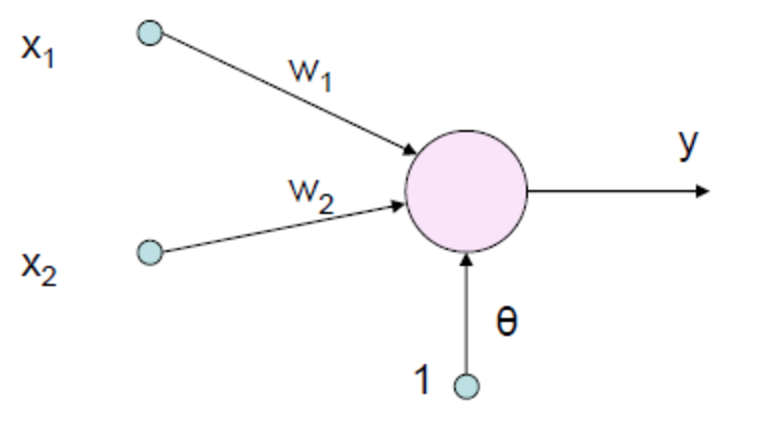
\includegraphics[width=0.25\textwidth]{img/psimple}
\end{center}

El aprendizaje supervisado se basa en un entrenamiento en el cual se provee al sistema con informacion de las entradas y de igual forma se proveen las salidas esperadas para cada entrada en particular.

Intuitivamente, el perceptron multicapa permite aproximar funciones, categorizar y encontrar patrones.

\begin{center}
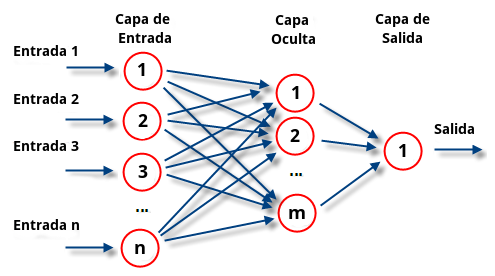
\includegraphics{img/pmulticapa}
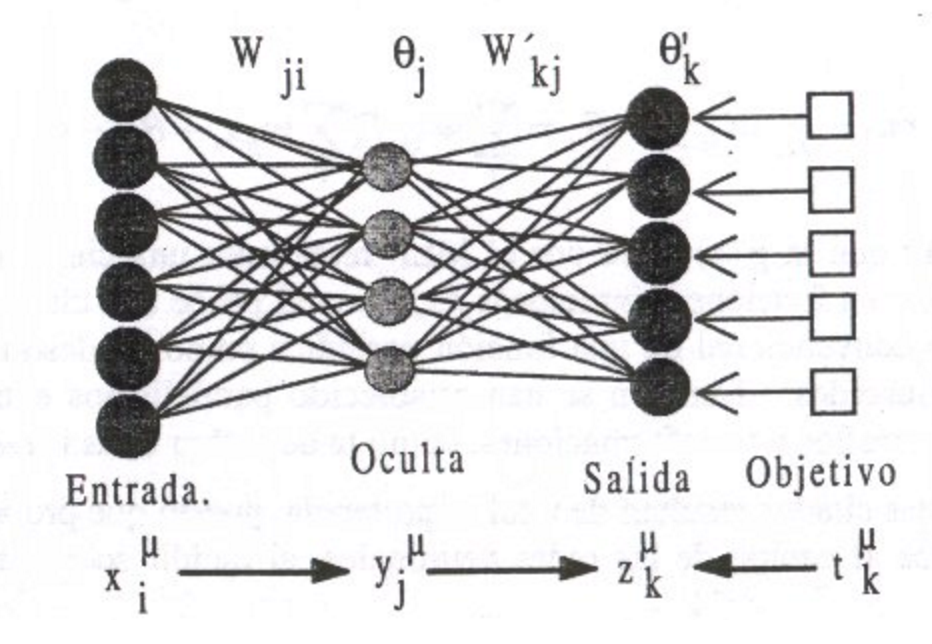
\includegraphics[width=0.35\textwidth]{img/pmulticapa2}
\end{center}

Las neuronas de la capa oculta usan como regla de propagacion la suma ponderada de las entradas con los pesos sinápticos $w_{ij}$ y sobre esa suma ponderada se aplica una funcion de transferencia de tipo sigmoide, que es acotada en respuesta.

\newpage
Grafico de funcion sigmoide:

\begin{center}
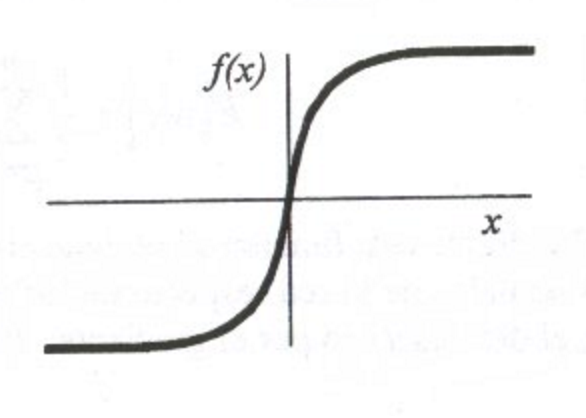
\includegraphics[width=0.30\textwidth]{img/sigmoide}
\end{center}

Sobre el aprendizaje, para este se suele usar en este tipo de redes recibe el nombre de backpropagation. Como funcion de coste global, se usa el error cuadratico medio. Es decir, que dado un par ($x_k$, $d_k$) correspondiente a la entrada k de los datos de entrenamiento y salida deseada asociada se calcula la cantidad.

Por otro lado, las capas pueden clasificarse en tres tipos:

\begin{enumerate}
\item \textbf{Capa de entrada:} Constituida por aquellas neuronas que introducen los patrones de entrada en la red. 
\item \textbf{Capas ocultas:} Formada por aquellas neuronas cuyas entradas provienen de capas anteriores y cuyas salidas pasan a neuronas de capas posteriores.
\item \textbf{Capa de salida:} Neuronas cuyos valores de salida se corresponden con las salidas de toda la red.
\end{enumerate}


En general la estructura de una neurona se puede representar de la siguiente manera:

\begin{center}
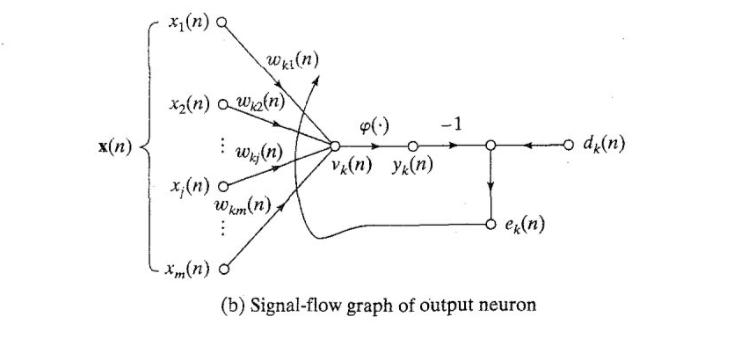
\includegraphics[width=0.6\textwidth]{img/neurona}
\end{center}

Podemos observar como los elementos mas importantes al vector de entrada de la neurona $(x_1,...,x_m)$, a los pesos correspondientes como $w_{ij}$, a la funcion de activacio y al elemento de salida. A partir de esta estructura basica la neurona puede mapear las entradas para obtener a la salida una respuesta deseada que pudiera pertenecer a alguna funcion a de terminar.


La funcion de activacion trata de simular el mecanismo que realiza el sistema de neuronas en el cerebro, que se basa en la exitacion de las neuronas hasta un cierto punto en el cual se pasa un umbral en el que dicha neurona dispara la informacion que le corresponde. Entre las diferentes funciones de activacion podemos encontrar la sigmoide.


Por otro lado el perceptron cuenta con un coeficiente de entrenamiento que indica que tanto varian los pesos entre iteracion e iteracion, por lo cual indica que tan lento o rapido la red se entrena.
\section{Detalles implementativos}
Utilizamos el lenguaje \textit{Python}, y seguimos el paradigma orientado a objetos. Creamos una clase \textit{Perceptrón Múltiple} que representa la red neuronal, y en otro archivo definimos la interfaz con el usuario. La clase se inicializa con los parámetros esperables de \textit{learning rate}, capas, etc., y mediante funciones públicas permite entrenar con datasets, con diversos métodos, predecir un output. 

Para ambos problemas a resolver, se usaron las mismas funciones, siendo diferentes la carga de los datos. 

Como función de activación usamos la sigmoidea bipolar. 

La interfaz y los detalles de cada ejercicio se explicará en secciones posteriores. 

Las funciones que se ofrecen son las siguientes:
\begin{itemize}
\item \textbf{activation} Calcula el output de al red dado un $X_{h}$
\item \textbf{correction} Calcula los $\Delta$ W dado un target $Z_{h}$
\item \textbf{adaptation} Aplica los $\Delta$ W 
\item \textbf{batch} 
\item \textbf{incremental}
\item \textbf{holdout} Dado un porcentaje, reserva un set para validación. 
\end{itemize}

Se pensó en implementar la técnica de \textit{early stopping} pero se evitó para no aumentar la complejidad del código.

\subsection{Algoritmos}
En esta sección describimos los pseudo-códigos de los algoritmos que utilizamos para resolver ambos ejercicios.
%Pseudocodigo de Activation
\begin{center}
\noindent\fbox{
\begin{minipage}{0.5\textwidth}
\begin{algorithm}[H]
 activation($X_h$)\;
 $Y_1$ = $X_h$\;
 \For{j de 2 a L}{
    $Y_j = f_j(Y_{j-1} * w_j)$\;
  }
  return $Y_l$\;
 \caption{Activation}
\end{algorithm}
\end{minipage}
}
\end{center}

%Pseudocodigo de Correction
\begin{center}
\noindent\fbox{
\begin{minipage}{0.5\textwidth}
\begin{algorithm}[H]
 correction($Z_k$)\;
  E = (Z-$Y_l$)\;
  e = $||E||^2$\;
  \For{j de L a 2}{
    $D = E * F_j^{'} (Y_{j-1}*W_j)$\;
    $dw_j = dw_j + \eta (Y_{j-1}^{T}*D)$\;
    $E = D*w_j^{t}$\;
  }
  return e\;
 \caption{Correction}
\end{algorithm}
\end{minipage}
}
\end{center}

%Pseudocodigo de Adaptation
\begin{center}
\noindent\fbox{
\begin{minipage}{0.5\textwidth}
\begin{algorithm}[H]
 adaptation()\;
  \For{j de 2 a L}{
    $W_j = W_j + dw_j$\;
    $dw_j = w_j + dw_j$\;
  }
 \caption{Adaptation}
\end{algorithm}
\end{minipage}
}
\end{center}

%Pseudocodigo de Trainning Batch
\begin{center}
\noindent\fbox{
\begin{minipage}{0.5\textwidth}
\begin{algorithm}[H]
 batch(X,Z)\;
  $e = 0$\;
  \For{h de 1 a P}{
    activation($X_h$)\;
    e = e + correction($Z_h$)\;
  }
  adaptation()\;
  return e\;
 \caption{Batch}
\end{algorithm}
\end{minipage}
}
\end{center}

%Pseudocodigo de Trainning Incremental
\begin{center}
\noindent\fbox{
\begin{minipage}{0.5\textwidth}
\begin{algorithm}[H]
 incremental(X,Z)\;
  $e = 0$\;
  \For{h de 1 a P}{
    activation($X_h$)\;
    e = e + correction($Z_h$)\;
    adaptation()\;
  }
  
  return e\;
 \caption{Incremental}
\end{algorithm}
\end{minipage}
}
\end{center}

%Pseudocodigo de Holdout
\begin{center}
\noindent\fbox{
\begin{minipage}{0.5\textwidth}
\begin{algorithm}[H]
 holdout($\epsilon$,T)\;
  $e_t = 1$\;
  $t = 0$\;
  $e_v = 1$\;
  v = ?? \;
  \While{$e_t > \epsilon $ y t $<$ T}{
    $e_t$ = trainning($Y_{[:v]}, Z_{[:v]}$)\;
    $e_v$ = testing($X_{[:v]}, Z_{[:v]}$)\;
    t = t+1
  }
  return $e_v,t$\;
 \caption{Holdout}
\end{algorithm}
\end{minipage}
}

\end{center}
\section{Problemas}
\subsection{Cancer de mamas}
Los datos son resultado de un examen que se realizan para diagnosticar cancer de mamas. Para cada paciente contamos con 10 caracteristicas de las imagenes de las celulas, entre estas caracteristicas contamos con diagnostico, radio, perimetro, textura, area, suavidad, etc. 

Cada una de estas entradas corrresponde a los datos de distintos pacientes, es importante remarcar que se cuenta con el atributo del diagnostico final quen indica si un tumor es benigno o maligno (0 y 1 respectivamente).

Sobre este primer dataset se buscara entrenar una red neuronal para poder predecir, dado un nuevo paciente con sus datos, si su estado sera el de tener cancer o no.

Este tipo de problemas se denomina un \textbf{problema de clasificacion}

Para resolver este problema decidimos utilizar un perceptron multicapa con una funcion de activacion sigmoidea bipolar. No utilizamos un perceptron simple debido a que este no siempre es capaz de generalizar y cualquier funcion que el simple sea capaz de aprender, el multicapa tambien lo hara.

Como primer medida, para mantener la estabilidad numerica del calculo, decidimos normalizar la entrada. Esto se debe a que al implementarse sobre aritmetica finita, los errores numericos tienden a propagarse mucho mas rapido cuando se aplica operaciones sobre numeros grandes que en los pequenos.

Por otro lado, al no conocer cual es el modelo optimo de redes neuronales para este problema, decidimos correr un algoritmo de busqueda para estimar cual es el numero apropiado de capas y neuronas. Tomando este resultado, intentamos mejorarlo analizando el comportamiento variando poco a poco las capas y analizando los graficos de error cometido y unidades equivocadas. Este proceso esta descripto con mas detalle en la \textbf{seccion de experimentacion} del ejercicio 1

\subsection{Eficiencia energetica}

En el siguiente problema contamos con los datos sobre la carga energetica para calefaccionar y refrigerar edificios en funcion de ciertas caractersisticas de los mismos.

El analisis se realizo tomando en cuenta edificios de diversas caracteristifcas, que difieren con respecto a la superficie y distribucion de las areas de reflejo, la orientacioon, etc.

Para cada edificio contamos con area de la superficie total, area de las paredes, area del techo, orientacion, area de reflejo total, etc.

Es importante remarcar que tambien contamos, para cada edifico del dataset, la cantidad de energio necersaria para realizar una calefaccion y refrigeracion adecuada.

Sobre este segundo dataset se buscara entrenar una red neuronal para poder aproximar la funcion que determina la cantidad de energia necesaria para
la calefaccion y refrigeracion de un edificio en funcion de los parametros de entrada. Es decir, es un problema de regresion.

Por esto mismo, tuvimos que normalizar el output target a valores en el rango [-1,1] para que podamos predecirlo con la función sigmoidea bipolar.

\emph{\color{red} FALTA AGREGAR DETALLES DE NUESTRA IMPLEMENTACION}
\section{Experimentación}
\subsection{Búsqueda de la mejor solucion}

\subsubsection{Ejercicio 1}
Para el ejercicio 1, implementamos un algoritmo simple para probar distintas ejecuciones y quedarnos con las soluciones que convergian. 

La idea general del algoritmo es iterar variando el modo de ejecucion (Sanger y Oja) y variando el \textbf{Learning Rate}. Por otro lado tambien modificamos a mano el parametro de epsilon para poder comparar y hacer la experimentacion. Es decir, para cada epsilon encontramos las mejores soluciones.

En el caso de \textbf{Sanger} se ejecuta variando el \textbf{Learning Rate} pero en caso de que una solucion converga, se corta, dado que una vez que se encuentra una solucion en Sanger esta es \textbf{la} solucion.

En el caso de \textbf{Oja} se ejecuta variando el \textbf{Learning Rate} y en caso de que converga guardamos la solucion y en caso de que no, no la guardamos.

El algoritmo para hacer estas pruebas es el siguiente:


\begin{lstlisting}[caption=pruebas]
	
	def pruebas(dataset,save_file,max_epochs=5000):
	best_params_oja = []
	best_params_sanger = -1
	for m in [0, 1]:
		for lrate in np.linspace(0.001, 0.1, 20):
			convergio = train_Ej1(dataset, save_file, 3, lrate, max_epochs,m)
			if convergio and not m:
				best_params_sanger = lrate
				break
			if convergio and m:
				best_params_oja.append(lrate)
	return best_params_sanger, best_params_oja

\end{lstlisting}

\subsubsection{Ejercicio 2}

\subsection{Ejercicio 1}

Como se explico anteriormente se corrio nuestro algoritmo de pruebas para encotnrar las mejores soluciones en cada modo. El algoritmo de pruebas es corrio con distintos \textbf{epsilons} y obtuvimos lo siguientes resultados:

\begin{tabular}{|l|l|l|}
\hline
Epsilon & Sanger & Oja \\ \hline
0.01           & -1      	& [0.001]  \\ \hline
0.015          & 0.001      & [0.001]   \\ \hline
0.02           & 0.001      & [0.001]   \\ \hline
0.05           & 0.001      & [0.001, 0.0062105263157894736, 0.011421052631578946]   \\ \hline
0.1            & 0.001      & [0.001, 0.006211, 0.0114211, 0.01664, 0.021843]   \\ \hline

\end{tabular}


En la tabla se puede ver para cada epsilon, los resultados obtenidos con cada algoritmo. En caso de Sanger si tiene un \textbf{-1} es porque no convergio a una solucion, en cambio, si converge se muestra el valor del Learning Rate. En el caso de Oja, el valor de la celda en la tabla es una lista con los Learning Rates que convergieron a una solucion.

En todos los casos se analizaron los graficos para ver que solucion es mejor que otra y pudimos ver que:

Con un epsilon de 0.1 en sanger obtuvimos un grafico como el siguiente:


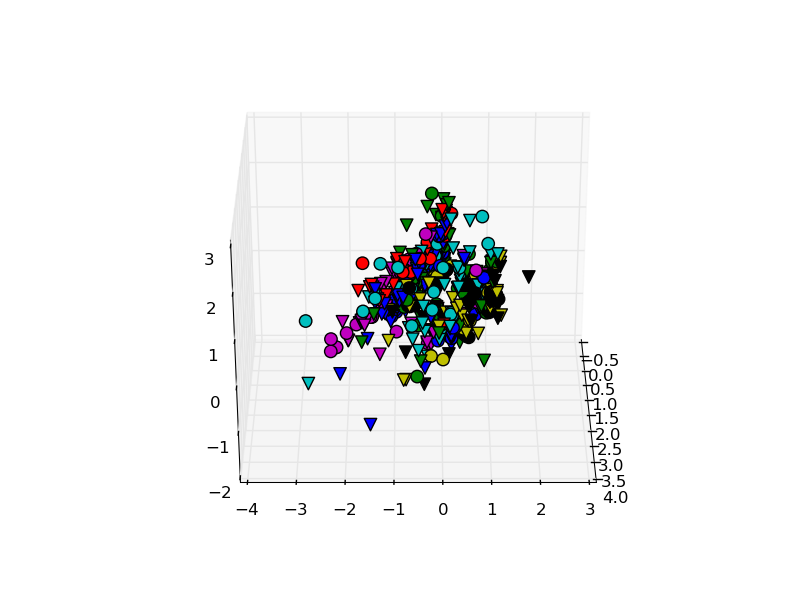
\includegraphics[width=0.5\textwidth]{img/ej1_sanger_01_20}
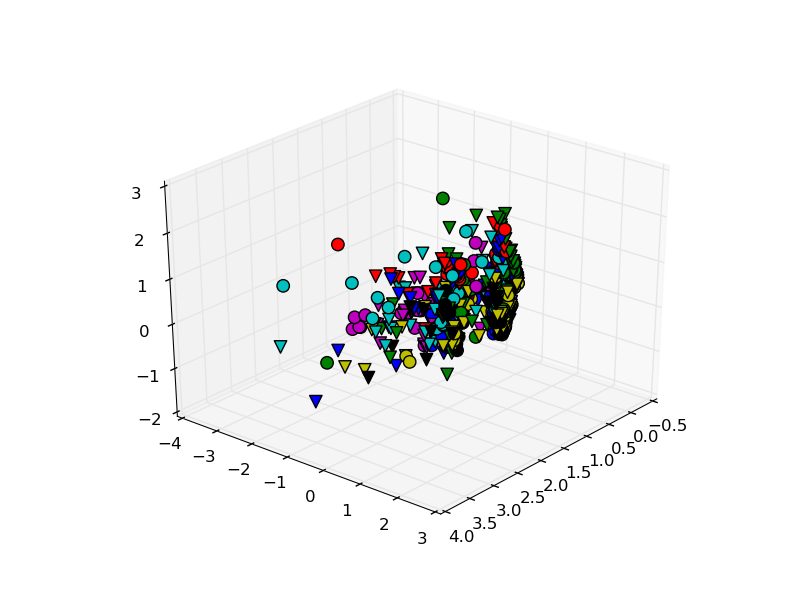
\includegraphics[width=0.5\textwidth]{img/ej1_sanger_01_40}
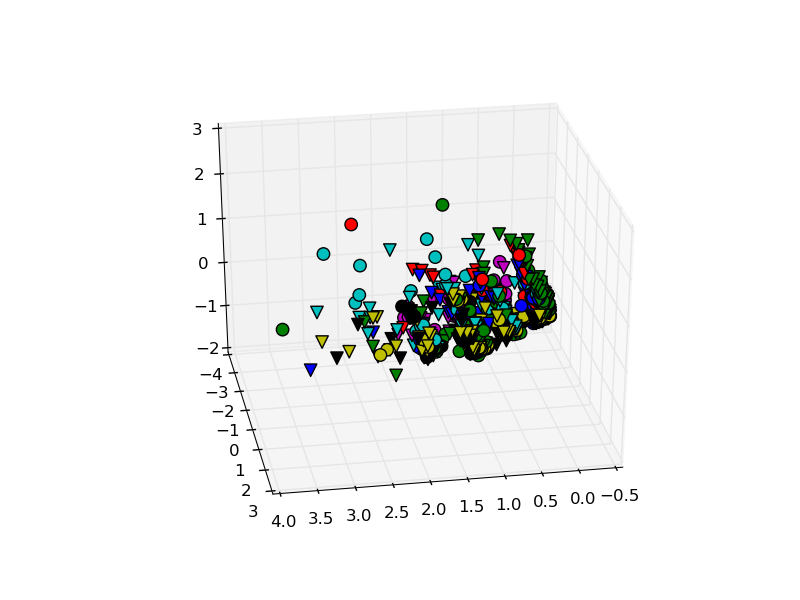
\includegraphics[width=0.5\textwidth]{img/ej1_sanger_01_80}
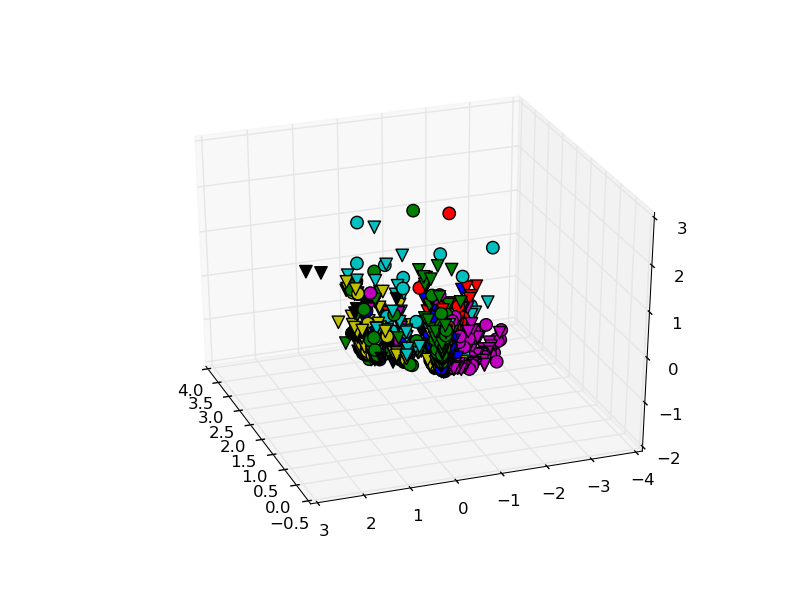
\includegraphics[width=0.5\textwidth]{img/ej1_sanger_01_160}
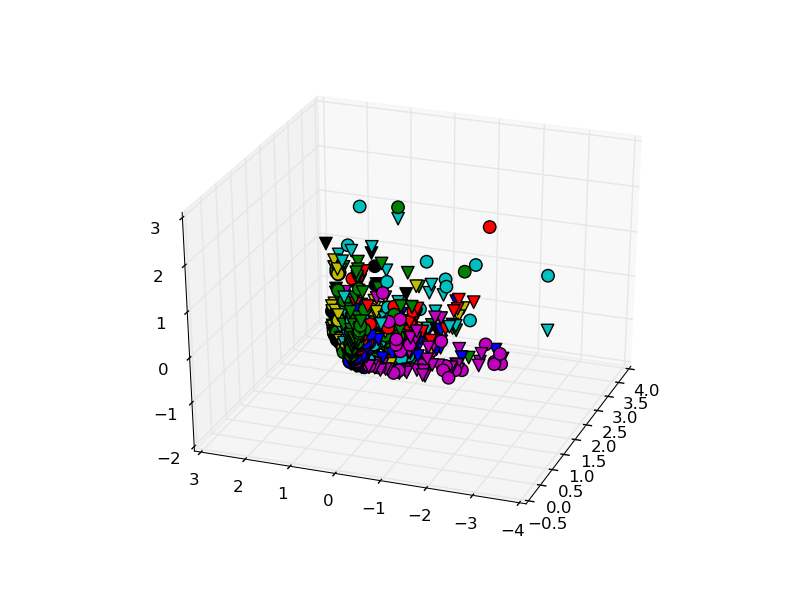
\includegraphics[width=0.5\textwidth]{img/ej1_sanger_01_200}
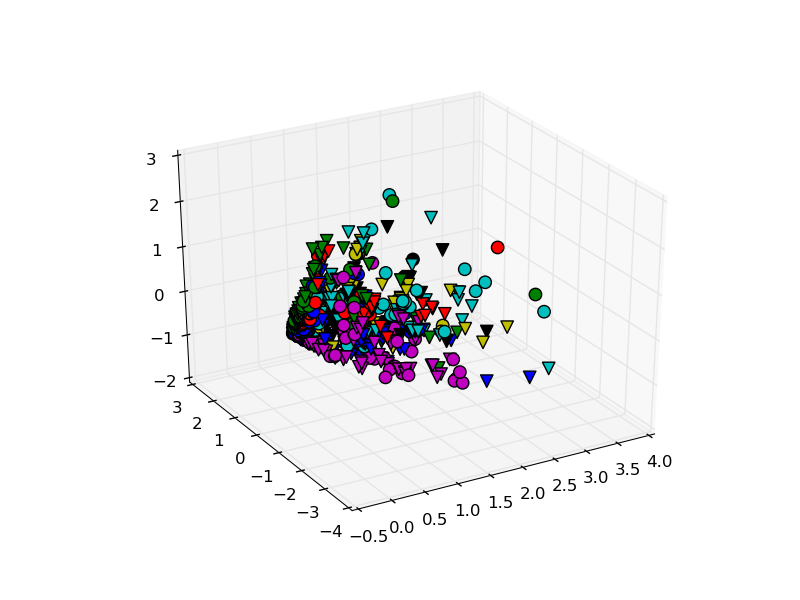
\includegraphics[width=0.5\textwidth]{img/ej1_sanger_01_240}


En este grafico lo que notamos muchos puntos estan dispersos, pero no solo dispersos, sino que son puntos dispersos de \textbf{distintos categorias}. 

Es dificil apreciar una agrupacion particular de un culor especifico, es decir, todos los colores estan un poco mezclados.

En particular el color amarillo se mezcla mucho con el verde, y el color rojo esta desparramado. 

Se nota tambien que el color violeta, al igual que el verde estan cerca de agruparse.

En algunos puntos se nota una mezcla intensa de color amarrilo y verde. Mientras que en otros lugares se nota esta mezcla pero de violeta, verde y azul.

Una particularidad de este grafico, es que el color rojo no resalta tanto y tiene un valor atipico.

con el mismo epsilon y con un learning rate de 0.001, en Oja obtuvimos 

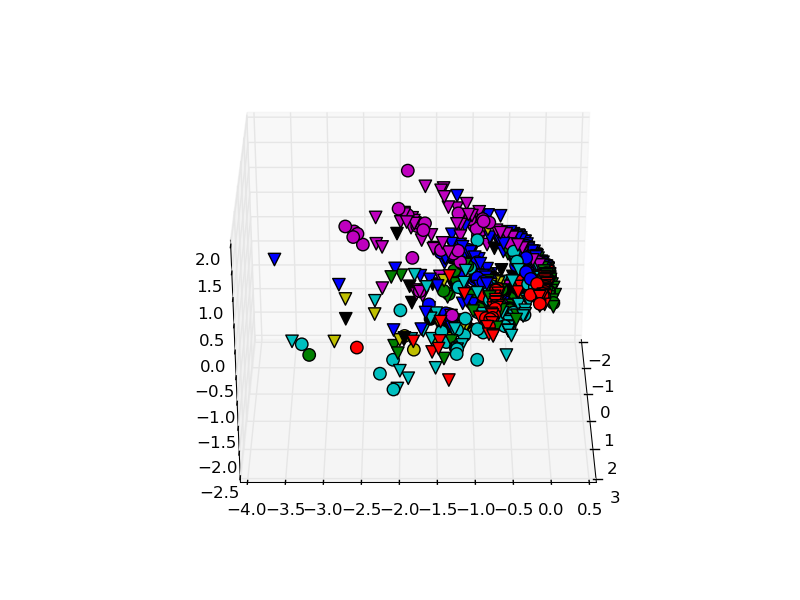
\includegraphics[width=0.5\textwidth]{img/ej1_oja_01_20}
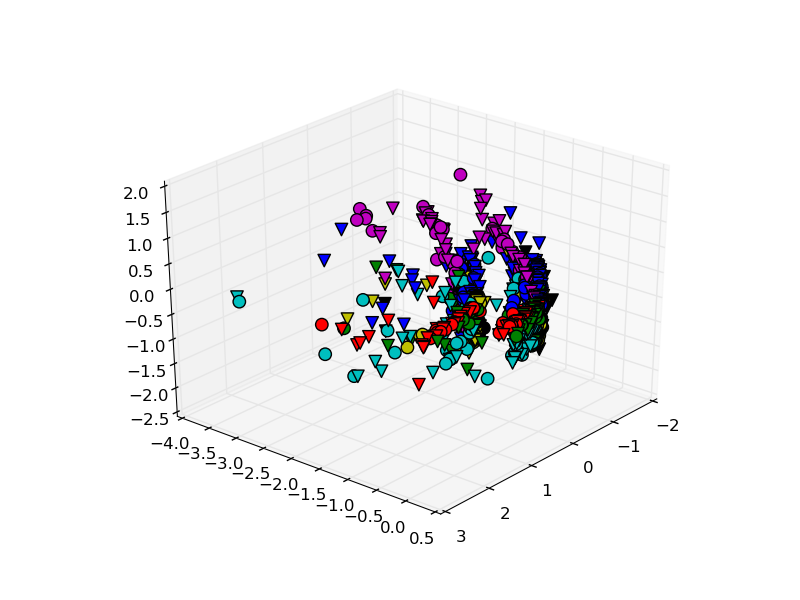
\includegraphics[width=0.5\textwidth]{img/ej1_oja_01_40}
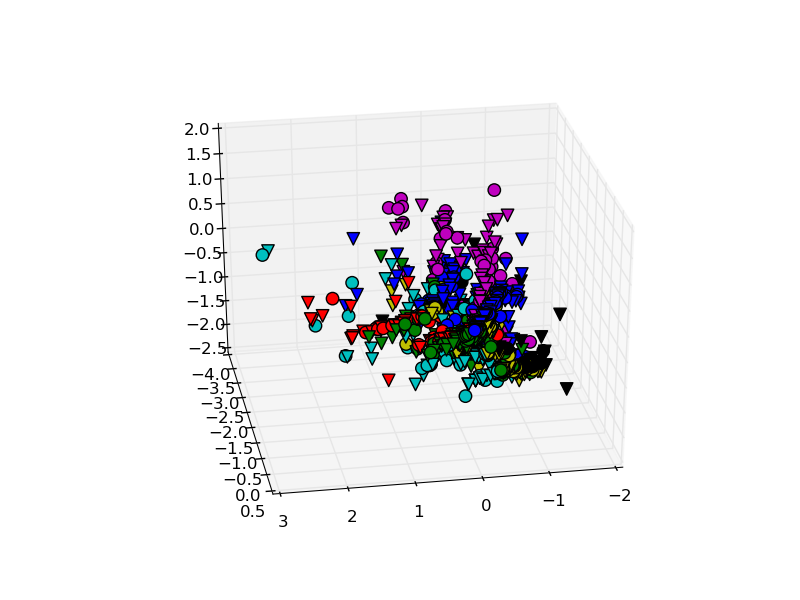
\includegraphics[width=0.5\textwidth]{img/ej1_oja_01_80}
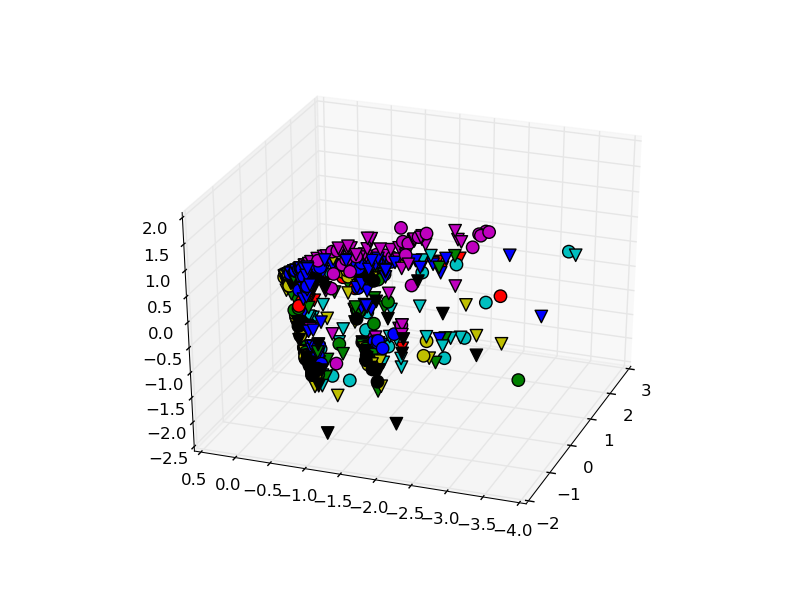
\includegraphics[width=0.5\textwidth]{img/ej1_oja_01_200}
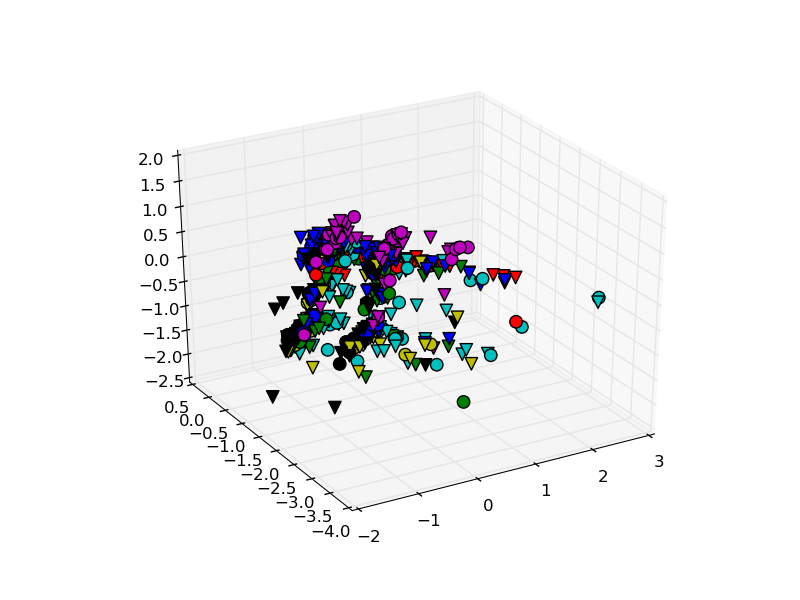
\includegraphics[width=0.5\textwidth]{img/ej1_oja_01_240}
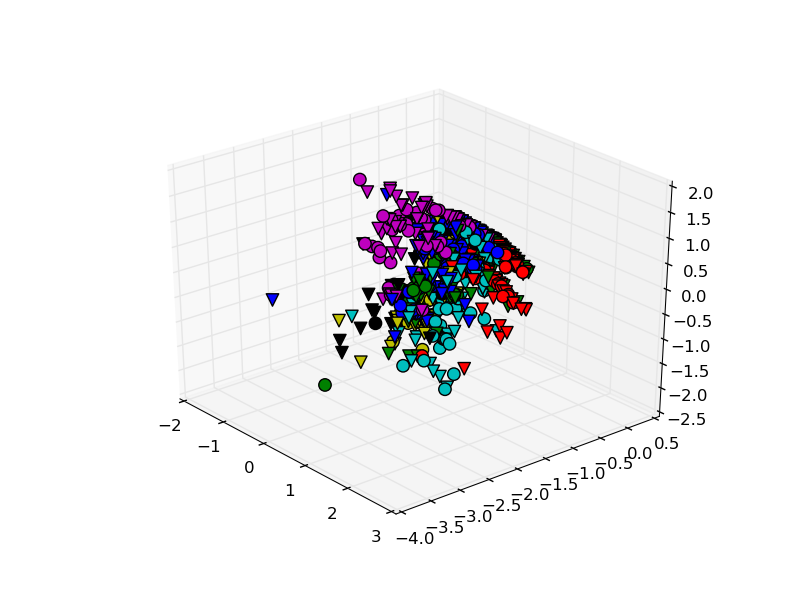
\includegraphics[width=0.5\textwidth]{img/ej1_oja_01_320}

En este grafico podemos observar donde grupos del mismoe lemento estan separados, como por ejemplo el violeta. Tambien observamos puntos outliers, dejando evidencia de que no llegaron a agruparse. 

En general se nota que las distintas categorias se mezclan intensamente y en casi ningun lado se llega a apreciar una categoria bien formada.

En algunas vistas (por ejemplo la ante ultima) vemos que no estan comprimidos, ni se nota una correlacion entre colores.

Como en la experimentacion anterior, se nota que tien mas problemas con el verde y el amarrillo que con el resto.


Por otro lado, analizando todos los graficos de las soluciones obtenidas deducimos que una mejora solucion (decision tomada analizando visualmente los graficos) es la siguiente:

Con un epsilon de 0.05 en sanger obtuvimos un grafico como el siguiente:


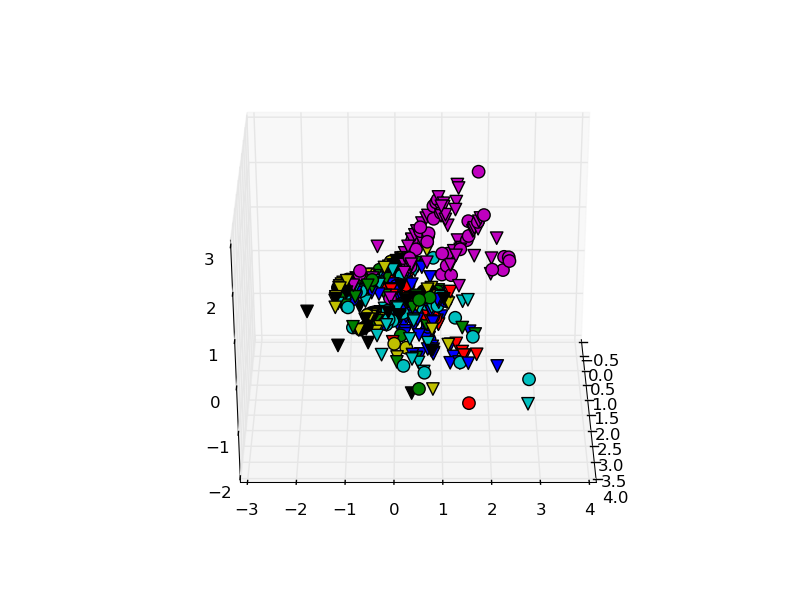
\includegraphics[width=0.5\textwidth]{img/ej1_sanger_005_20}
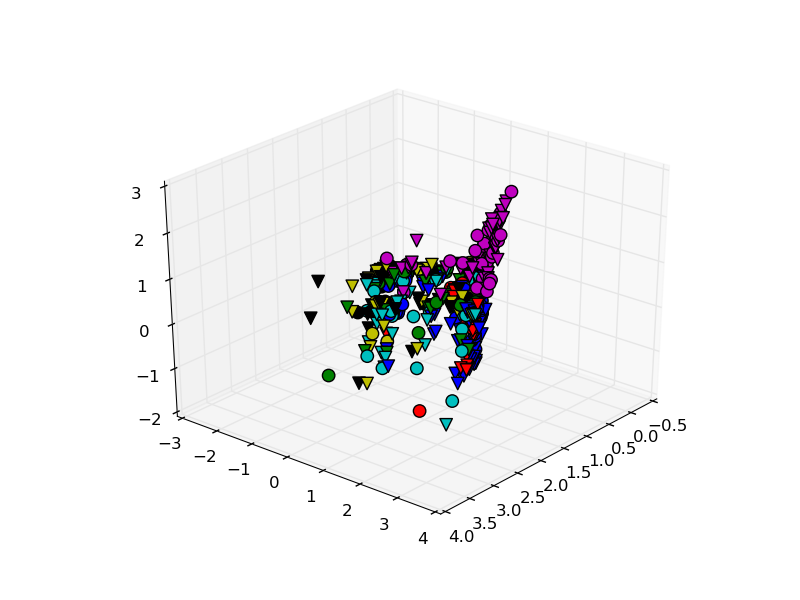
\includegraphics[width=0.5\textwidth]{img/ej1_sanger_005_40}
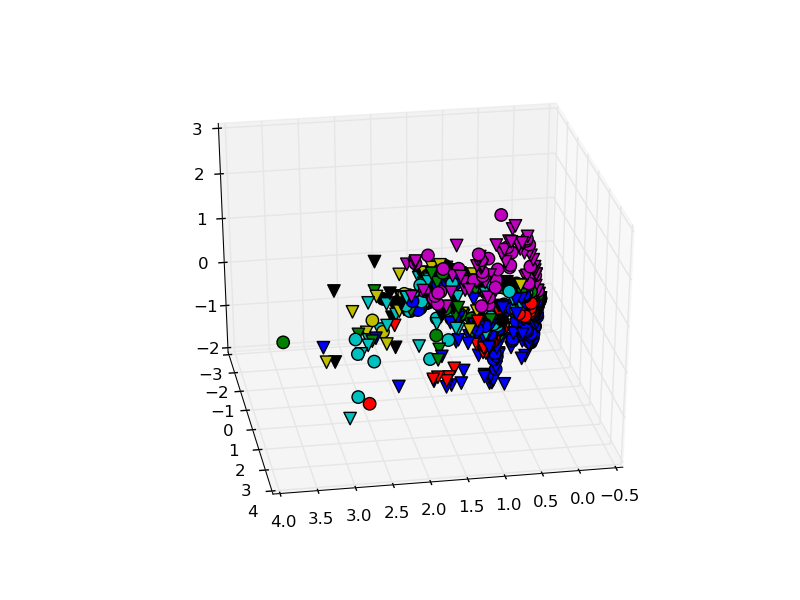
\includegraphics[width=0.5\textwidth]{img/ej1_sanger_005_80}
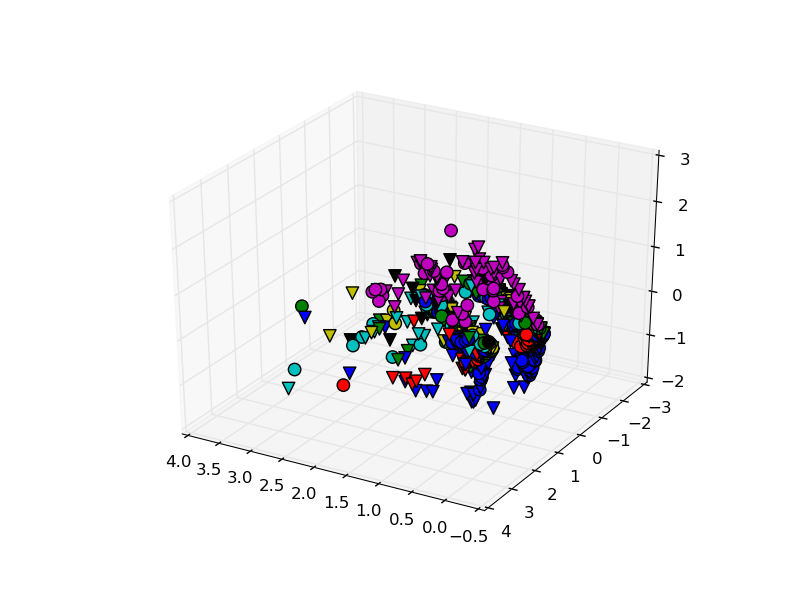
\includegraphics[width=0.5\textwidth]{img/ej1_sanger_005_120}
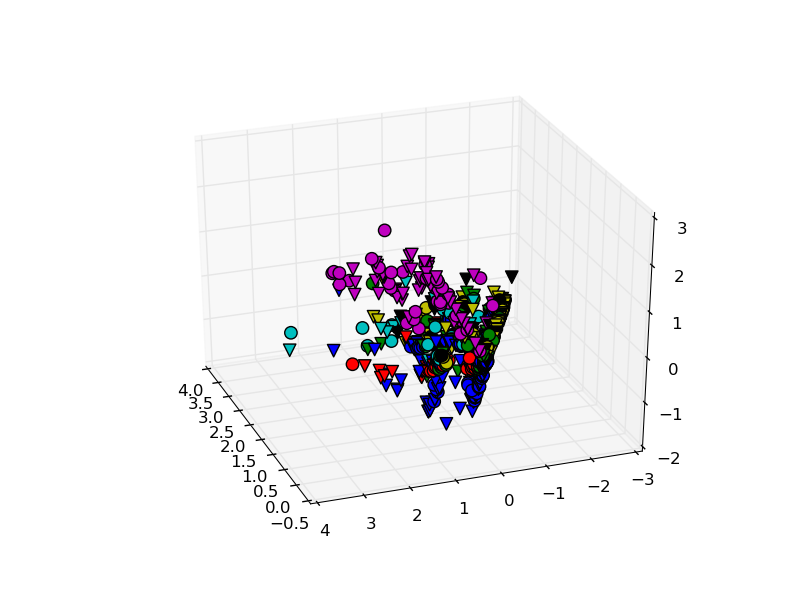
\includegraphics[width=0.5\textwidth]{img/ej1_sanger_005_160}
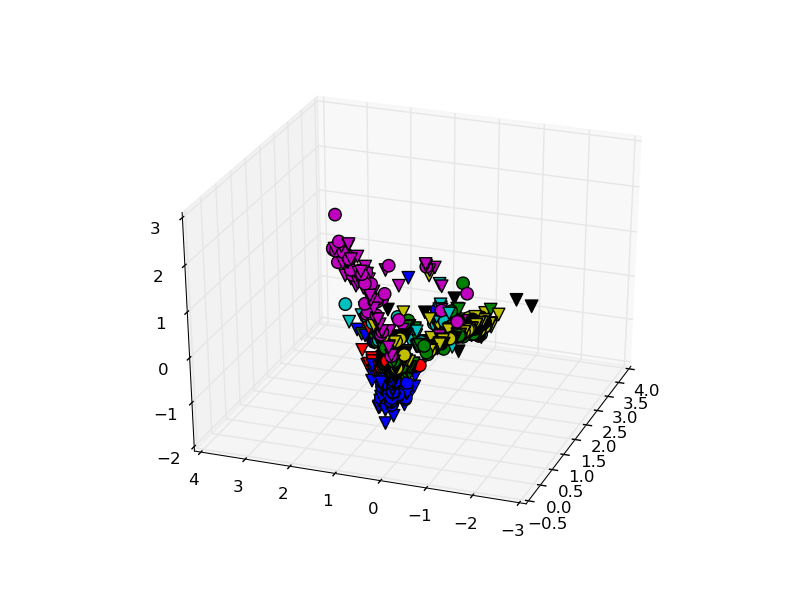
\includegraphics[width=0.5\textwidth]{img/ej1_sanger_005_200}


En estos graficos notamos claramente que el color violeta se separa en una categoria bien definida. 

Por otro lado, en estos graficos, a diferencia de los anteriores, se puede notar como el color azul tambien esta definiendo mejor la discretizacion que en experimentos anteriores.

En el ultimo grafico podems notar claramente la semaparacion entre el violeta y el azul, pero de igual manera vemos que el verde y amarrillo siguen mezclados, por suerte, no tanto como antes, pero siguen mezclando.

Con un epsilon de 0.05 y un Learning Rate de 0.001 en Oja obtuvimos:

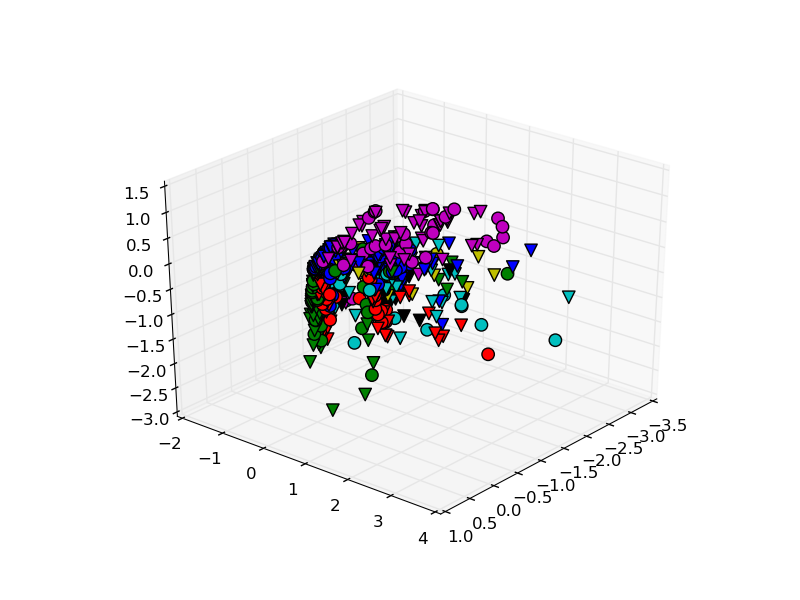
\includegraphics[width=0.5\textwidth]{img/ej1_oja_005_20}
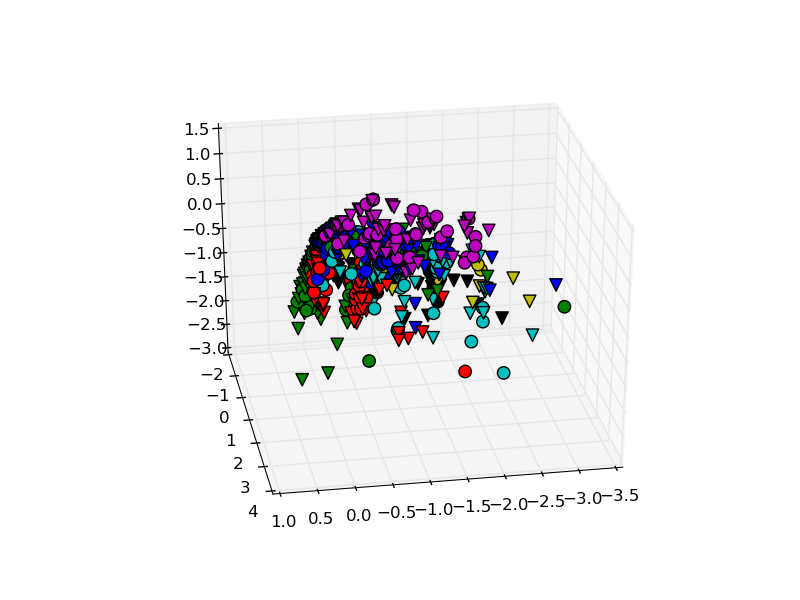
\includegraphics[width=0.5\textwidth]{img/ej1_oja_005_80}
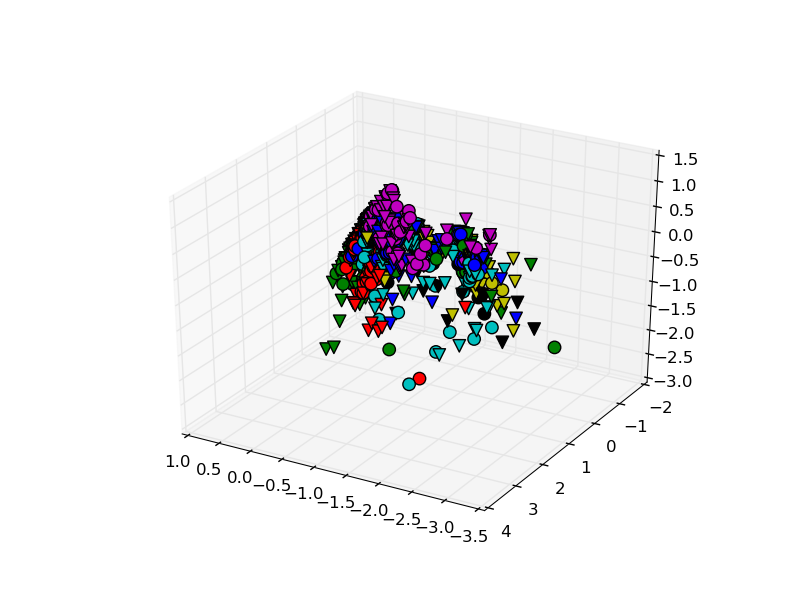
\includegraphics[width=0.5\textwidth]{img/ej1_oja_005_120}
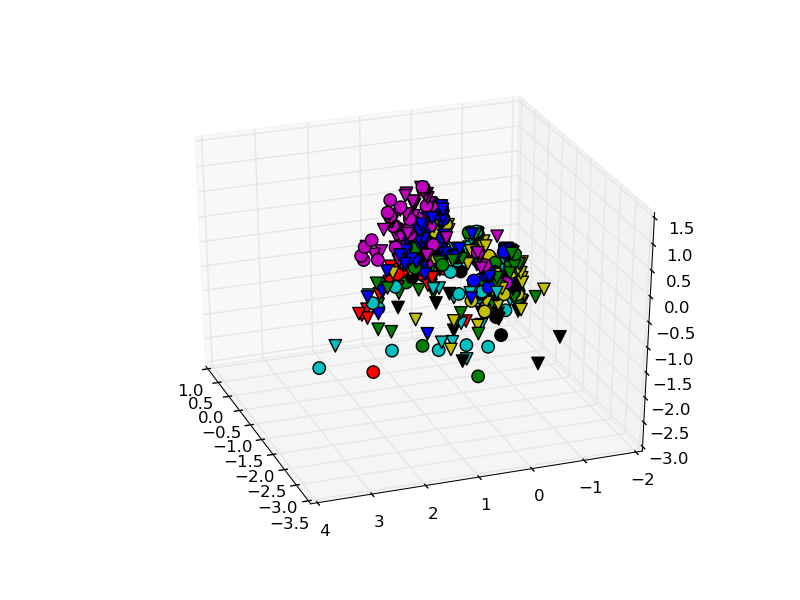
\includegraphics[width=0.5\textwidth]{img/ej1_oja_005_160}
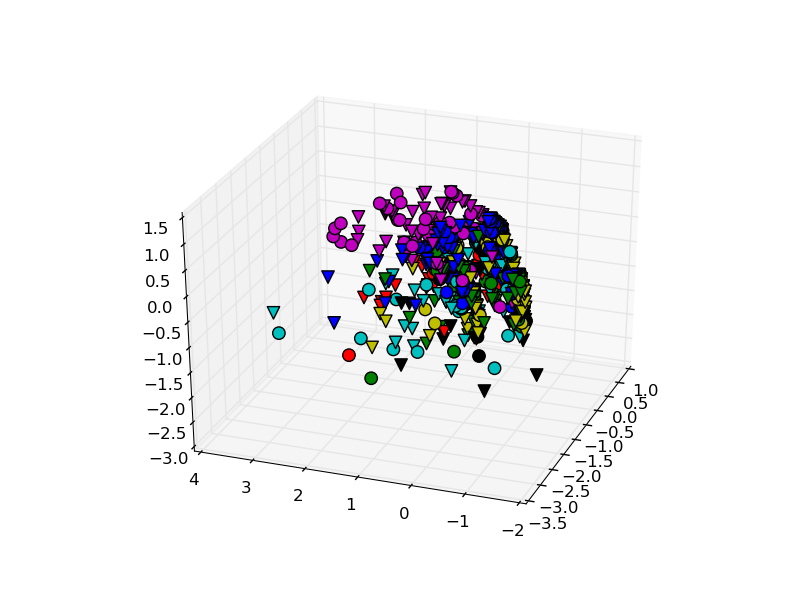
\includegraphics[width=0.5\textwidth]{img/ej1_oja_005_200}
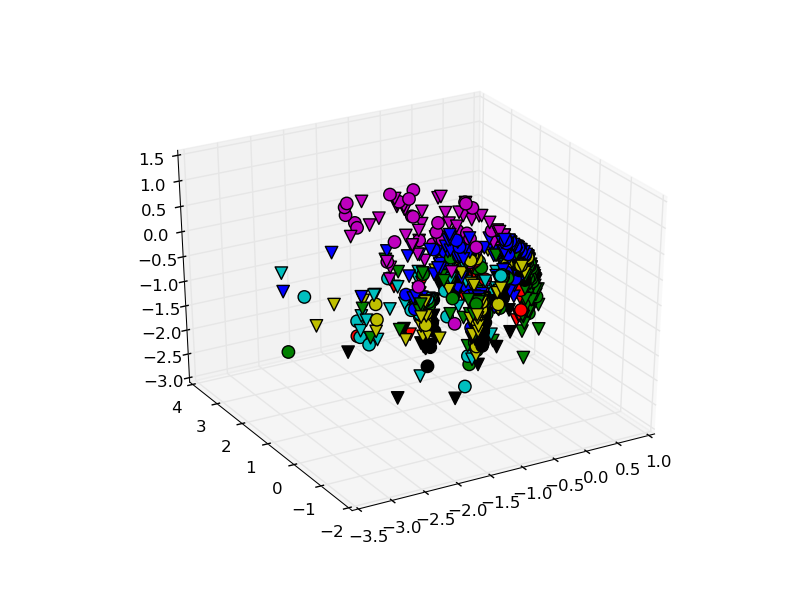
\includegraphics[width=0.5\textwidth]{img/ej1_oja_005_240}

En este grafico vemos, como en el anterior que el color violeta se agrupa de forma correcta.

Del mismo modo que el color azul. Lo mas notable de este grafico es que el color rojo empieza a aparecer en una especie de \textbf{categorizacion}, detalle que antes no pasaba. 

Otro factor importante es que el color verde y el amarillo no se mezclan tanto como en graficos anteriores.

\subsubsection{Conclusion}

Luego de analizar los graficos y resultados del ejercicio 1, podemos concluir que al contrario de lo que esperabamos, en lugar de agruparse en distintas esferas bien definidas, los resultados dieron mas heterogeneos.

Concluimos que la mejor solucion es la ultima proporcionada por Oja (epsilon: 0.05 y learning rate: 0.001), debido a las justificaciones explicadas previamente. En general, se observa que las categorias estan mejor agrupadas.

En general, notamos que los gr\'aficos poseen unas lineas de colores bien definidas, esto es, asumiendo que las categorias son ortoganles, porque cada categor\'ia trata de ajustarce a una dimension, y al haber 9 categorias no alcanzan lsa dimenseiones, por lo tanto vemos estos solapamientos.

\subsection{Ejercicio 2}

Para el ejercicio 2, implementamos un algoritmo para probar distintas dimensiones (cuadradas) de espacio de salida e ir variando los \textbf{Sigma} y \textbf{Epocas}, para ver como influyen, en manera general, en la agrupacion. Para ello, cada una de las corridas se guardan los graficos resultantes y se analiza su comportamiento.

Una vez conseguidos todos los graficos hicimos un analisis observando cual tiene una mejor agrupacion, al igual que en el ejercicio 1, pero esta vez en el plano.


\begin{lstlisting}[caption=pruebas]
	
def prueba():
	file="tp2_training_dataset.csv"
	train_data = np.genfromtxt(file, delimiter=',',usecols=range(1,857))
	train_data=train_data[:600]
	test_data  = np.genfromtxt(file, delimiter=',',usecols=range(0,857))
	if not os.path.exists("imgs/ej2"):
		os.makedirs("imgs/ej2")
	for epoca in [5,10,25,100,500,1000,1500]:
		for M in [3,5,9,20,30,40]:
			for sigma in np.linspace(0.001, 1, 20):
				img_name="imgs/ej2/train_M_"+str(M)+"_sigma_"+str(sigma)+"_epocas_"+str(epoca)+".png"
				print img_name
				red = som(M, M,sigma)
				red.train(train_data,epoca)
				graficador(red,test_data[:600],img_name)
				img_name="imgs/ej2/test_M_"+str(M)+"_sigma_"+str(sigma)+"_epocas_"+str(epoca)+".png"
				graficador(red,test_data[600:],img_name)

\end{lstlisting}

Como se explic\'o anteriormente se corri\'o nuestro algoritmo de pruebas para encontrar las mejores soluciones. El algoritmo de pruebas corrio con estos \textbf{M1} y \textbf{M2}:

\begin{tabular}{|l|l|}
\hline
M1 & M2 \\ \hline
3 & 3 \\ \hline
5 & 5 \\ \hline
9 & 9 \\ \hline
20 & 20 \\ \hline
30 & 30 \\ \hline
40 & 40 \\ \hline
\end{tabular}

y estas epocas
\begin{tabular}{|l|}
\hline
Epocas\\ \hline
100 \\ \hline
500 \\ \hline
1000 \\ \hline
1500 \\ \hline
\end{tabular}

Los resultados de el entrenamiento(izquieda) vs test (derecha) comparando diferentes dimensiones y una epoca de 500. Dado que fueron resultados similares, se exponen los m\'as representativos.

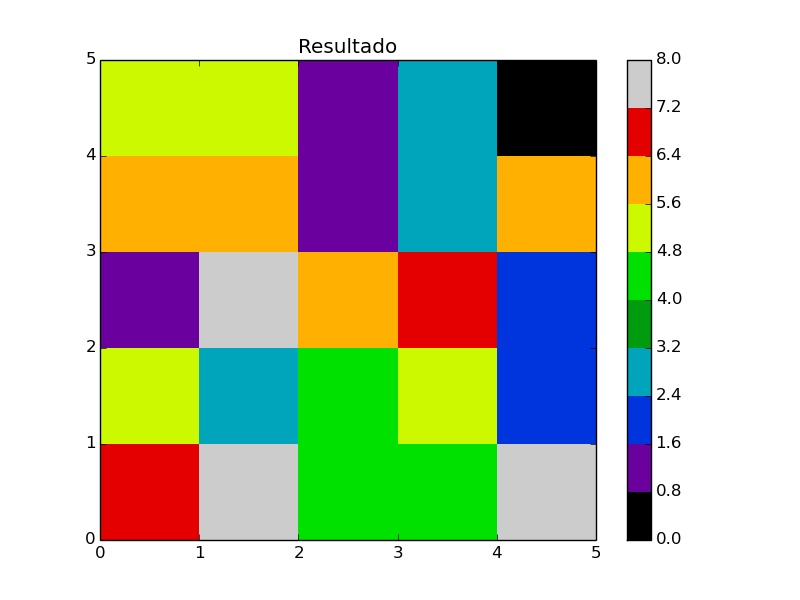
\includegraphics[width=0.5\textwidth]{img/ej2_train_M_5_lrate_001_epocas_500}
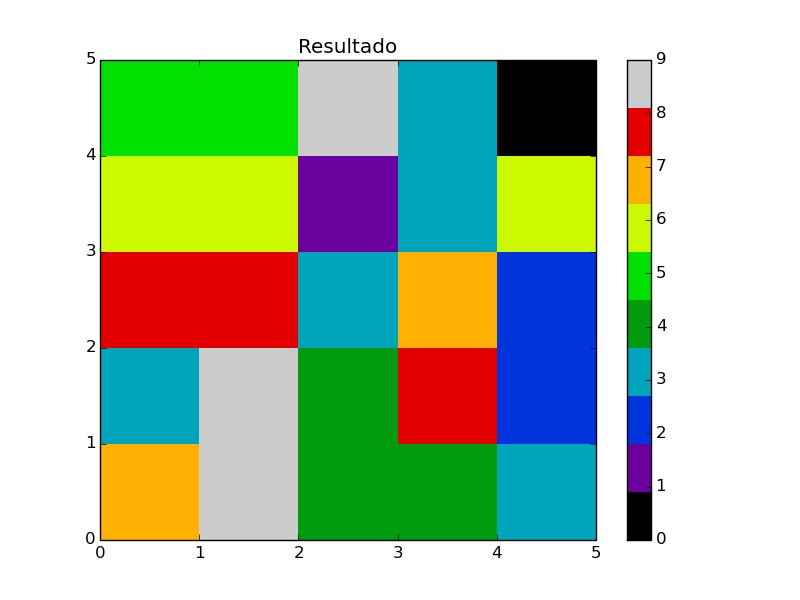
\includegraphics[width=0.5\textwidth]{img/ej2_test_M_5_lrate_001_epocas_500}
{\footnotesize Entrenamiento vs Testing Red 5x5 Learning Rate 0.001 Epocas 500\par}

Como se puede observar a simple vista, la clasificacion obtenida por el test no es consistente con la obtenida en el entrenamiento. Esto puede deberse a que la reduccion de 900 dimensiones a solo 5x5 comprime demasiado la informacion y no es suficiente para agruparlas. Este mismo efecto se observo en las redes de 3x3.

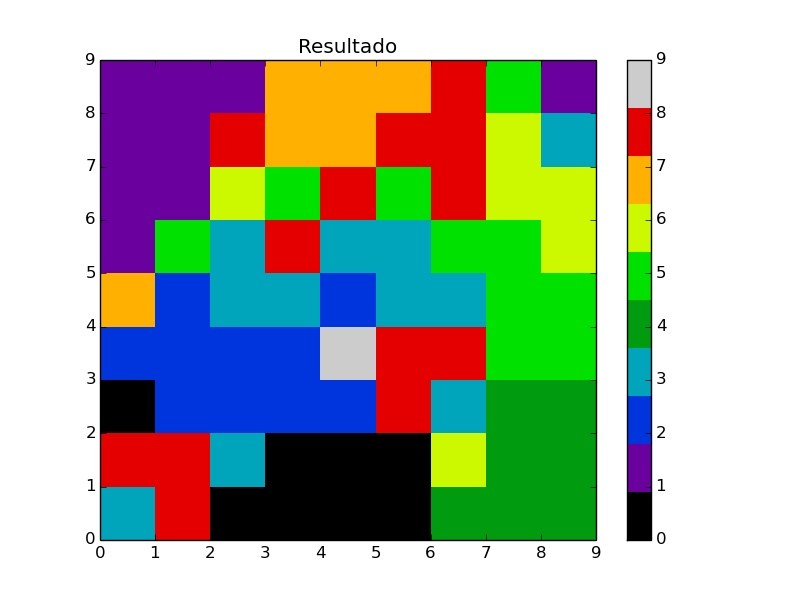
\includegraphics[width=0.5\textwidth]{img/ej2_train_M_9_lrate_001_epocas_500}
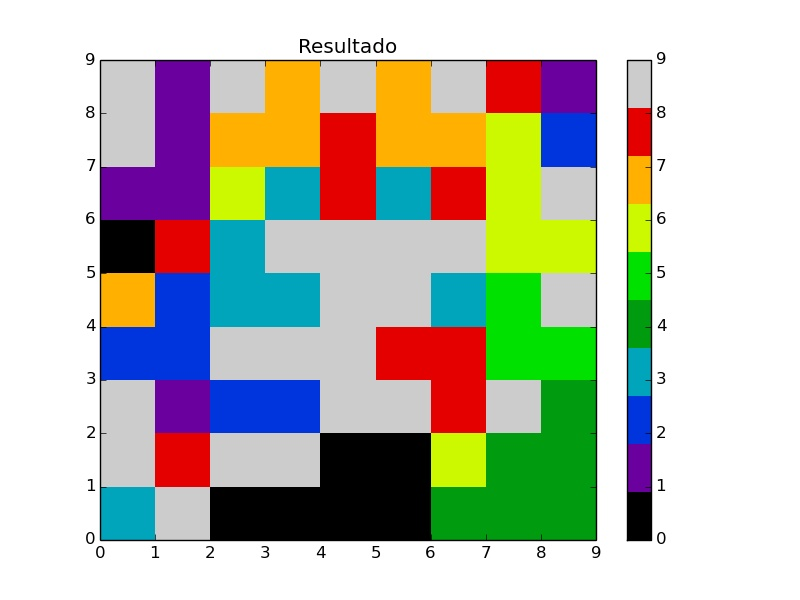
\includegraphics[width=0.5\textwidth]{img/ej2_test_M_9_lrate_001_epocas_500}
{\footnotesize Entrenamiento vs Testing Red 9x9 Learning Rate 0.001 Epocas 500\par}

A diferencia del anterior, se empiezan a notar grupos bien definidos, a excepcion del rojo. Este grupo debe compartir caracteristicas de los otros ocho y por este motivos se deben estar mezclando. 

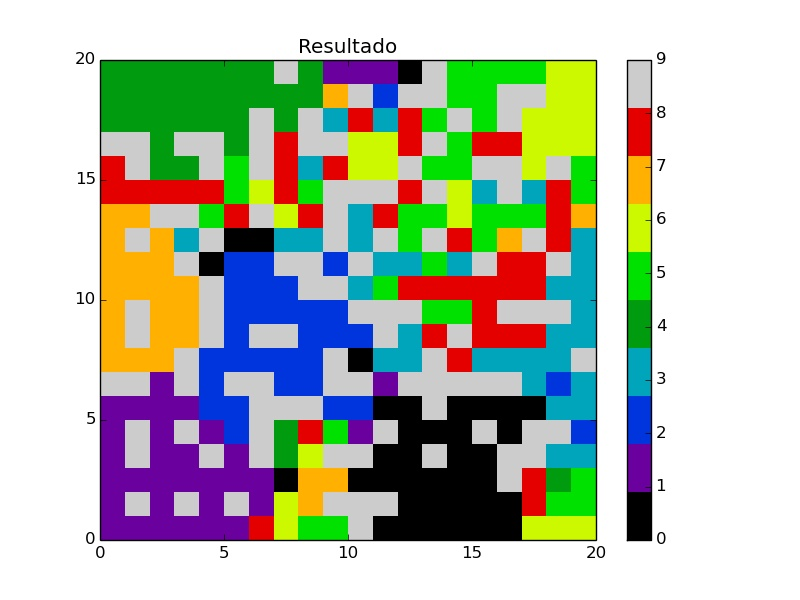
\includegraphics[width=0.5\textwidth]{img/ej2_train_M_20_lrate_001_epocas_500}
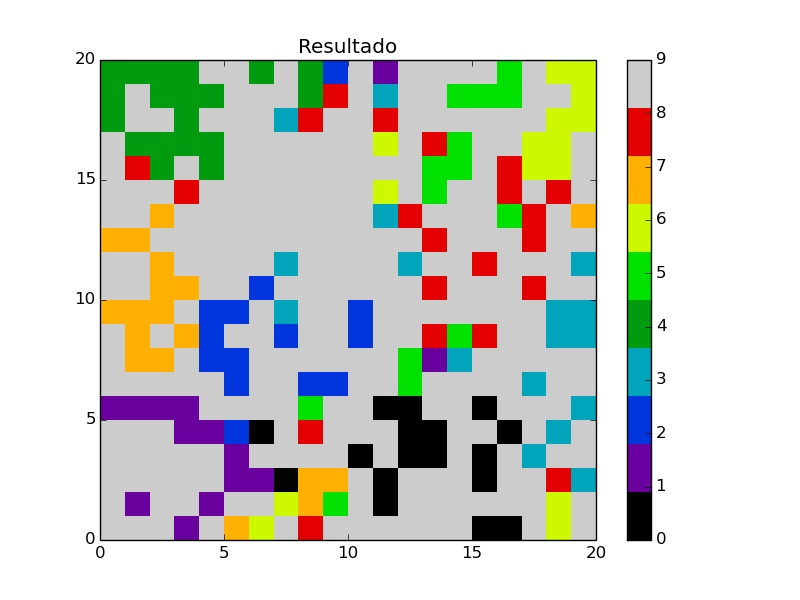
\includegraphics[width=0.5\textwidth]{img/ej2_test_M_20_lrate_001_epocas_500}
{\center \footnotesize Entrenamiento vs Testing Red 20x20 Learning Rate 0.001 Epocas 500\par}

Como se esperaba, al incrementar el espacio de salida y reducir la compresion, los colores se separan m\'as y se agrupan mejor. Se nota una mejora sobre el rojo pero los grupos de color aun presentan puntos de color diferentes.

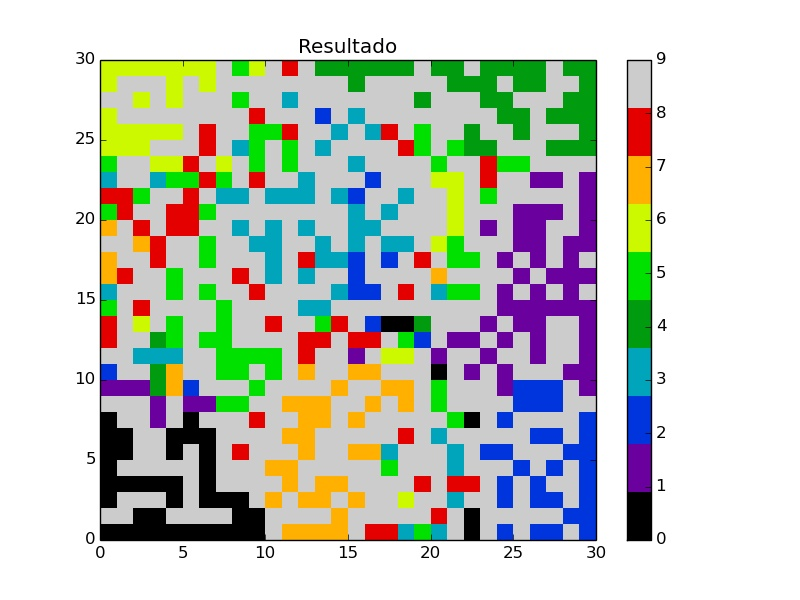
\includegraphics[width=0.5\textwidth]{img/ej2_train_M_30_lrate_001_epocas_500}
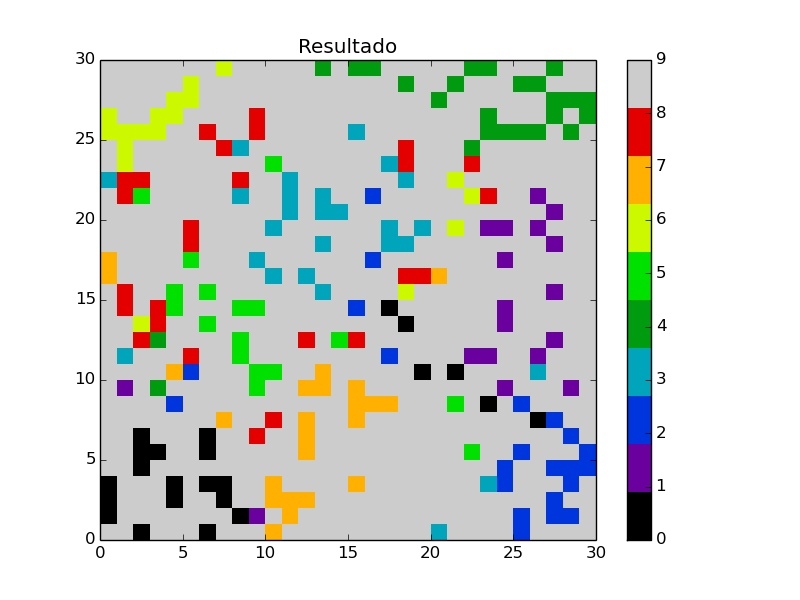
\includegraphics[width=0.5\textwidth]{img/ej2_test_M_30_lrate_001_epocas_500}
{\footnotesize Entrenamiento vs Testing Red 30x30 Learning Rate 0.001 Epocas 500\par}

En este espacio, donde cada punto tiene su equivalente con el espacio de entrada, se aprecia la misma tendencia de grupos que en el caso anterior de 20x20. Pero a su vez, se notan una gran cantidad de neuronas sin activar, sobre todo en la fronteras de los grupos verde oscuro, violeta, azul y negro. El grupo naranja queda definido en la zona central inferior y bastante aislado del resto. Adem\'as, notamos que el color rojo establece un cord\'on alrededor del color verde claro y el turquesa, por lo que esta clasificaci\'on es una categoria que implicar\'ia varias disciplinas. Suponemos que esta es la raz\'on por la cual redes de menor tama\~no no pudieron agrupar bien el color rojo.

Un patron notable en todas las pruebas es que los grupos nunca aparecen en la misma posici\'on, incluso con los mismos par\'ametros. Esto puede deberse a la aleatoriedad para inicializarlos

Ahora compararemos los resultados de el entrenamiento(izquierda) vs test (derecha) en base al sigma inicial. Si bien se experimento con todas las dimensiones, dado que los mejores resultados para el caso anterior se obtuvieron con dimension 20x20 y 30x30 solo se mostrar\'an los resultados obtenidos por estas instancias.


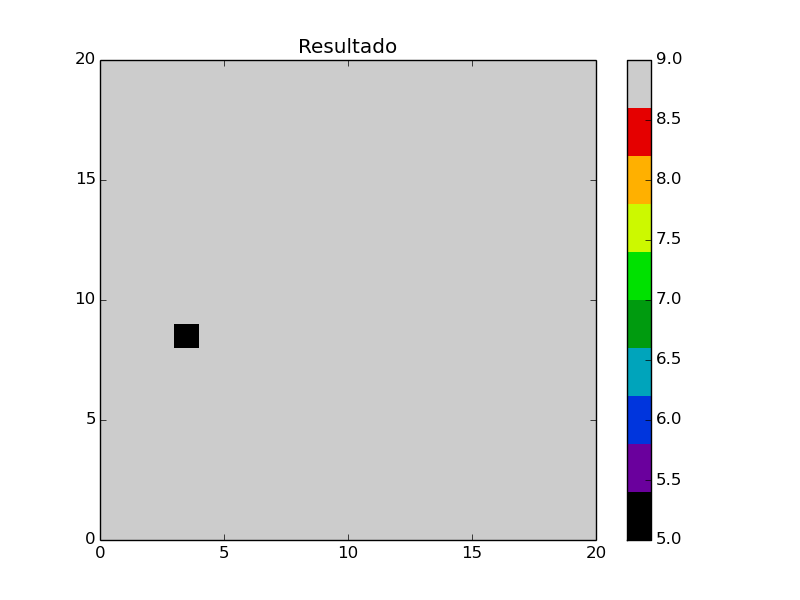
\includegraphics[width=0.5\textwidth]{img/EJ2_Sigma/train_M_20_sigma_0_001_epocas_5}
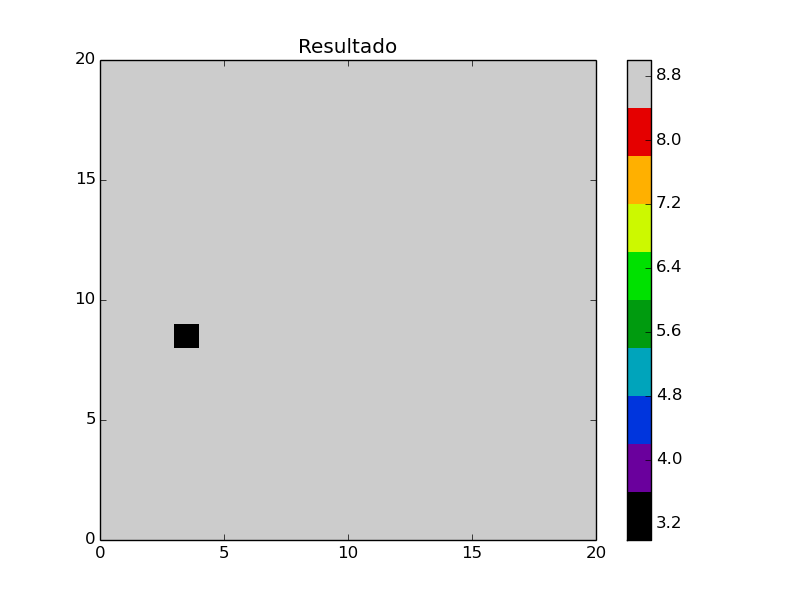
\includegraphics[width=0.5\textwidth]{img/EJ2_Sigma/test_M_20_sigma_0_001_epocas_5}
{\center \footnotesize Entrenamiento vs Testing Red 20x20 Sigma 0.001 Epocas 10\par}

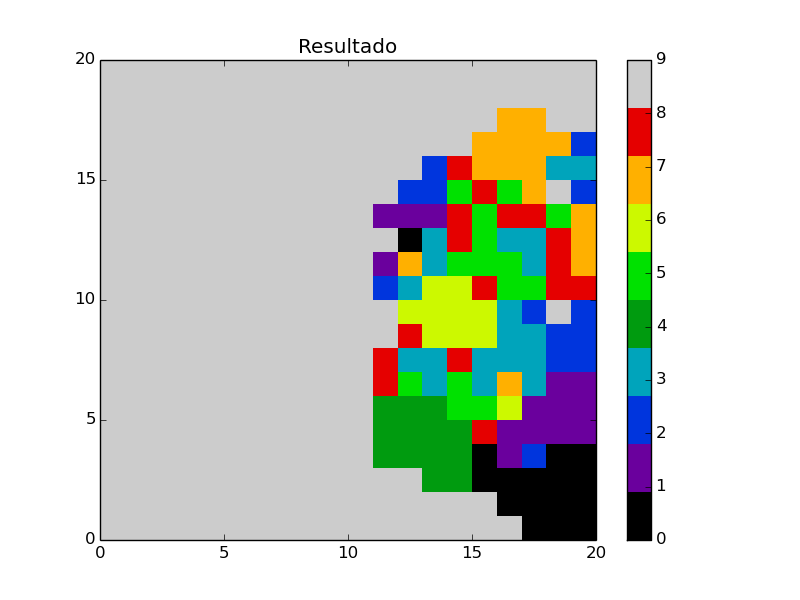
\includegraphics[width=0.5\textwidth]{img/EJ2_Sigma/train_M_20_sigma_1_25075_epocas_5}
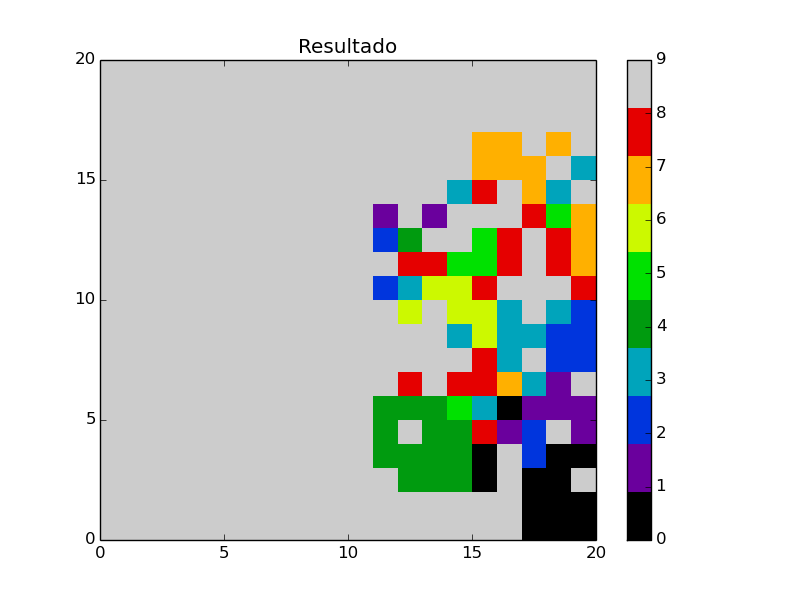
\includegraphics[width=0.5\textwidth]{img/EJ2_Sigma/test_M_20_sigma_1_25075_epocas_5}
{\center \footnotesize Entrenamiento vs Testing Red 20x20 Sigma 1.25075 Epocas 10\par}

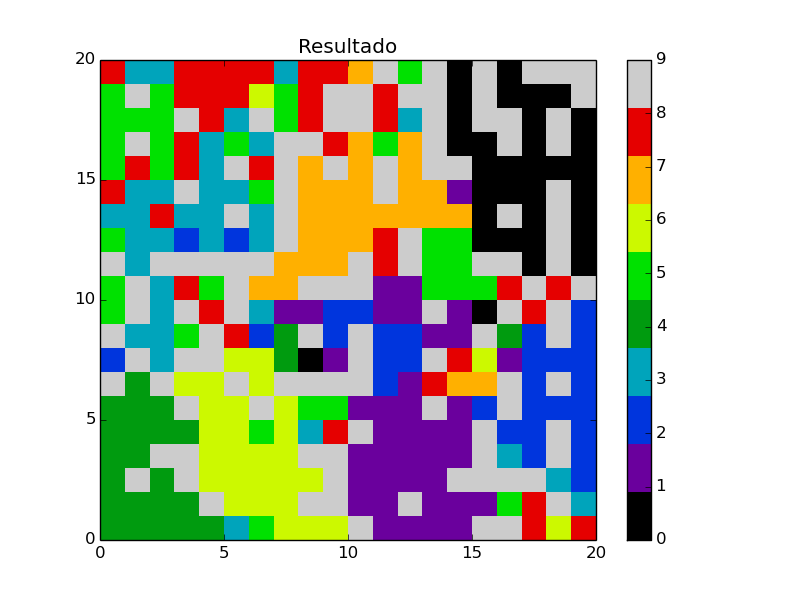
\includegraphics[width=0.5\textwidth]{img/EJ2_Sigma/train_M_20_sigma_2_5005_epocas_5}
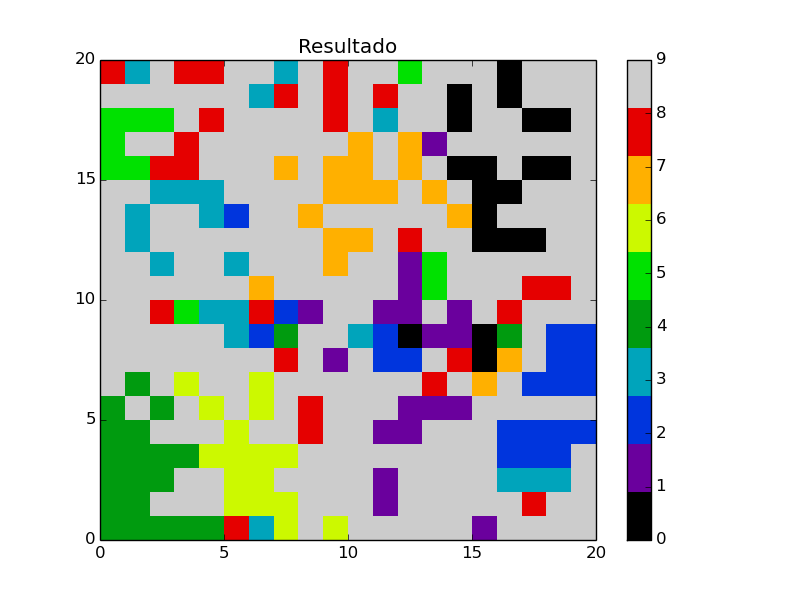
\includegraphics[width=0.5\textwidth]{img/EJ2_Sigma/test_M_20_sigma_2_5005_epocas_5}
{\center \footnotesize Entrenamiento vs Testing Red 20x20 Sigma 2.5005 Epocas 10\par}

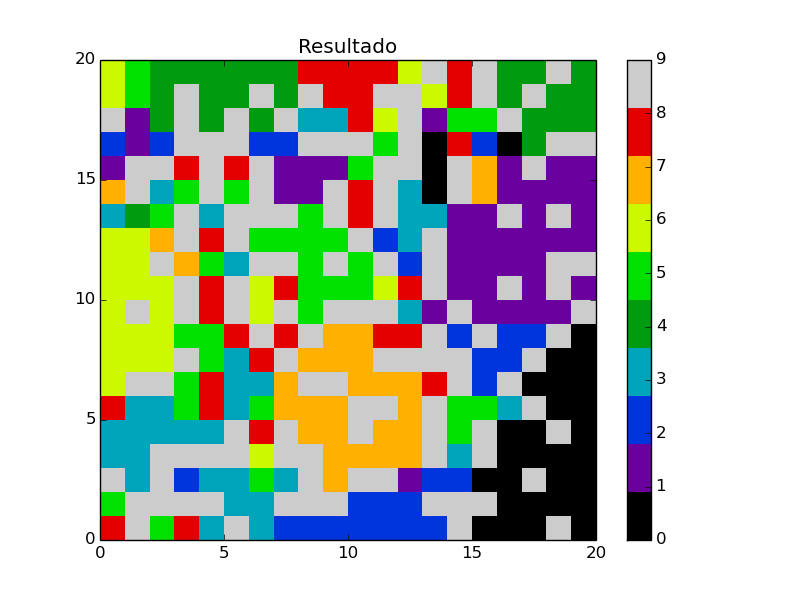
\includegraphics[width=0.5\textwidth]{img/EJ2_Sigma/train_M_20_sigma_3_75025_epocas_5}
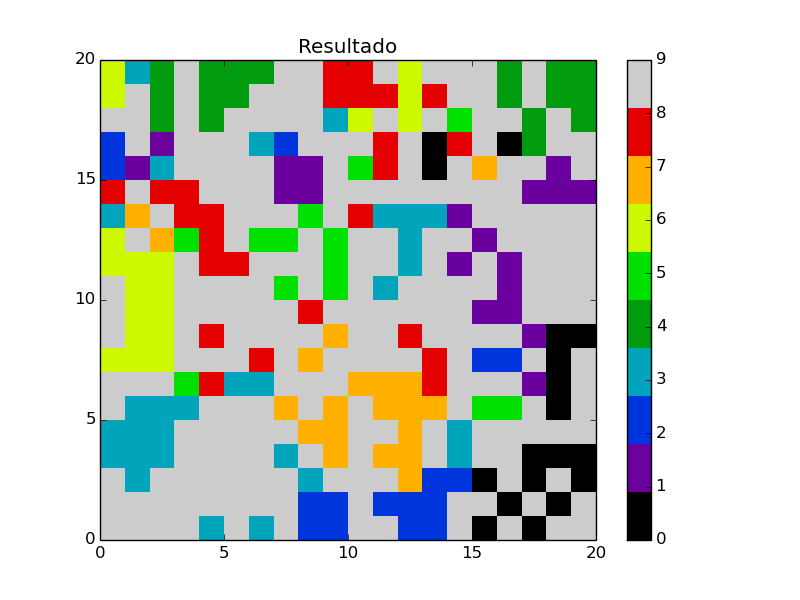
\includegraphics[width=0.5\textwidth]{img/EJ2_Sigma/test_M_20_sigma_3_75025_epocas_5}
{\center \footnotesize Entrenamiento vs Testing Red 20x20 Sigma 3.75025 Epocas 10\par}

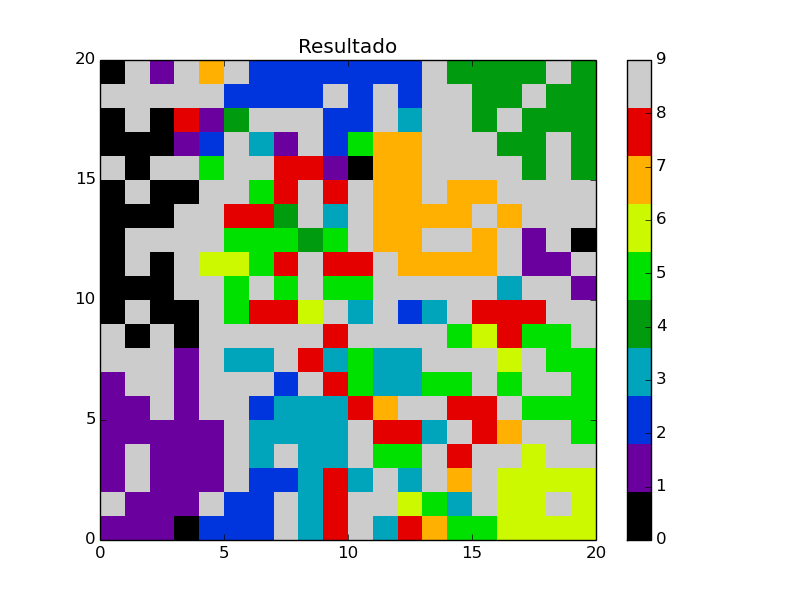
\includegraphics[width=0.5\textwidth]{img/EJ2_Sigma/train_M_20_sigma_5_0_epocas_5}
\includegraphics[width=0.5\textwidth]{img/EJ2_Sigma/test_M_20_sigma_5_0_epocas_5}
{\center \footnotesize Entrenamiento vs Testing Red 20x20 Sigma 5 Epocas 10\par}

Este comportamiento de agrandamiento de zonas de activacion comienza a notarse a partir de redes de tamaño 9. Vemos que el sigma influye en la velocidad de \"desparramiento\" y mejora la separacion cuanto mas grande es.

\includegraphics[width=0.5\textwidth]{img/EJ2_Sigma/train_M_30_sigma_0_001_epocas_5}
\includegraphics[width=0.5\textwidth]{img/EJ2_Sigma/test_M_30_sigma_0_001_epocas_5}
{\center \footnotesize Entrenamiento vs Testing Red 30x30 Sigma 0.001 Epocas 5\par}

\includegraphics[width=0.5\textwidth]{img/EJ2_Sigma/train_M_30_sigma_1_25075_epocas_5}
\includegraphics[width=0.5\textwidth]{img/EJ2_Sigma/test_M_30_sigma_1_25075_epocas_5}
{\center \footnotesize Entrenamiento vs Testing Red 30x30 Sigma 1.25075 Epocas 5\par}

\includegraphics[width=0.5\textwidth]{img/EJ2_Sigma/train_M_30_sigma_2_5005_epocas_5}
\includegraphics[width=0.5\textwidth]{img/EJ2_Sigma/test_M_30_sigma_2_5005_epocas_5}
{\center \footnotesize Entrenamiento vs Testing Red 30x30 Sigma 2.5005 Epocas 5\par}

\includegraphics[width=0.5\textwidth]{img/EJ2_Sigma/train_M_30_sigma_3_75025_epocas_5}
\includegraphics[width=0.5\textwidth]{img/EJ2_Sigma/test_M_30_sigma_3_75025_epocas_5}
{\center \footnotesize Entrenamiento vs Testing Red 30x30 Sigma 3.75025 Epocas 5\par}

\includegraphics[width=0.5\textwidth]{img/EJ2_Sigma/train_M_30_sigma_5_0_epocas_5}
\includegraphics[width=0.5\textwidth]{img/EJ2_Sigma/test_M_30_sigma_5_0_epocas_5}
{\center \footnotesize Entrenamiento vs Testing Red 30x30 Sigma 5 Epocas 5\par}

Ahora compararemos los resultados de el entrenamiento(izquierda) vs test (derecha) en base al tiempo de entrenamiento.

\includegraphics[width=0.5\textwidth]{img/Ej2_Epocas/train_M_20_sigma_3_75025_epocas_5}
\includegraphics[width=0.5\textwidth]{img/Ej2_Epocas/test_M_20_sigma_3_75025_epocas_5}
{\center \footnotesize Entrenamiento vs Testing Red 20x20 Sigma 3.75025 Epocas 5\par}

\includegraphics[width=0.5\textwidth]{img/Ej2_Epocas/train_M_20_sigma_3_75025_epocas_10}
\includegraphics[width=0.5\textwidth]{img/Ej2_Epocas/test_M_20_sigma_3_75025_epocas_10}
{\center \footnotesize Entrenamiento vs Testing Red 20x20 Sigma 3.75025 Epocas 10\par}

\includegraphics[width=0.5\textwidth]{img/Ej2_Epocas/train_M_20_sigma_3_75025_epocas_25}
\includegraphics[width=0.5\textwidth]{img/Ej2_Epocas/test_M_20_sigma_3_75025_epocas_25}
{\center \footnotesize Entrenamiento vs Testing Red 20x20 Sigma 3.75025 Epocas 25\par}

Ahora vemos

\includegraphics[width=0.5\textwidth]{img/Ej2_Epocas/train_M_30_sigma_3_75025_epocas_5}
\includegraphics[width=0.5\textwidth]{img/Ej2_Epocas/test_M_30_sigma_3_75025_epocas_5}
{\center \footnotesize Entrenamiento vs Testing Red 30x30 Sigma 3.75025 Epocas 5\par}

\includegraphics[width=0.5\textwidth]{img/Ej2_Epocas/train_M_30_sigma_3_75025_epocas_10}
\includegraphics[width=0.5\textwidth]{img/Ej2_Epocas/test_M_30_sigma_3_75025_epocas_10}
{\center \footnotesize Entrenamiento vs Testing Red 30x30 Sigma 3.75025 Epocas 10\par}

\includegraphics[width=0.5\textwidth]{img/Ej2_Epocas/train_M_30_sigma_3_75025_epocas_25}
\includegraphics[width=0.5\textwidth]{img/Ej2_Epocas/test_M_30_sigma_3_75025_epocas_25}
{\center \footnotesize Entrenamiento vs Testing Red 30x30 Sigma 3.75025 Epocas 25\par}


Si bien no hay una mejora en calidad de soluci\'on, es necesario aclarar que aunque terminen en la misma cantidad de epocas, el tiempo de computo de la solucion de la red de 30x30 es mucho mayor que la de 20x20. Por este motivo, la corrida de la red de 40x40 no se pudo realizar para mediciones mayores a 500 epocas.

\subsubsection{Conclusion}

Luego de analizar los graficos y resultados del ejercicio 2, podemos concluir que las dimensiones de la red no solo influyen en la calidad de la solucion sino tambien en el tiempo de calculo de la misma. 

En base a todo lo anterior, decidimos que la mejor solucion es una red de 30x30 con un learning rate de 0.01 y 100 epocas de entrenamiento. Esta red provee una buena clasificacion y balancea el costo en tiempo.

Esperabamos que el learning rate alterara significativamente el mapeo. Sin embargo, al utilizar la funcion sigma
eta = t ** (- 1/2) y sigma = (M2/2)* (t ** (-1/3)), creemos que acorto mucho el campo de vecinos que modifica la unidad ganadora, por lo cual, el cambio producido fue poco.


\section{Entregable}
\subsection{Contenido del entregable}
Lorem ipsum dolor sit amet, consectetur adipisicing elit, sed do eiusmod
tempor incididunt ut labore et dolore magna aliqua. Ut enim ad minim veniam,
quis nostrud exercitation ullamco laboris nisi ut aliquip ex ea commodo
consequat. Duis aute irure dolor in reprehenderit in voluptate velit esse
cillum dolore eu fugiat nulla pariatur. Excepteur sint occaecat cupidatat non
proident, sunt in culpa qui officia deserunt mollit anim id est laborum.

\subsection{Modo de ejecución}


\subsubsection{Ejercicio 1}


La manera de ejecutar el programa dado es la siguiente:

En caso de querer entrenar la red sera:

\begin{verbatim}
$ python main.py < archivo_entrada > < archivo_red_salida > -train < lrate > 
                                                   < max_epochs > < method >    
\end{verbatim}

Donde:

\begin{enumerate}
\item archivo\_entrada: archivo de dataset.
\item archivo\_red\_salida: archivo donde se guardara la red.
\item lrate: Coeficiente de aprendizaje.
\item max\_epochs: Maxima cantidad de epocas permitidas.
\item method: 
\begin{enumerate}
\item -s: Sanger
\item -o: Oja
\end{enumerate}
\end{enumerate}

Por ejemplo: 

Si queremos ejecutar el ejercicio 1 entrenandolo con el dataset \textbf{tp2\_training\_dataset.csv}, guardando la red en el archivo 
\textbf{red} con un learning\_rate de \textbf{0.01}, con un espacio de salida de \textbf{3}, con una cantidad maxima de epocas de \textbf{10000} y con el modo \textbf{Sanger} seria:

\begin{verbatim}
$ python main.py tp2_training.dataset.csv  red -train 0.01 10000 -s
\end{verbatim}

En caso de querer cargar una red ya guardada seria:

\begin{verbatim}
$ python main.py < archivo_entrada > < nombre_red_in > -load
\end{verbatim}

Donde:

\begin{enumerate}
\item archivo\_entrada: archivo de dataset.
\item nombre\_red\_in: nombre de la red a cargar.
\end{enumerate}

Por ejemplo, si queremos cargar la red llamada \textbf{red} con el dataset \textbf{tp2\_training\_dataset.csv} seria:

\begin{verbatim}
$  python main.py tp2_training_dataset.csv red -load
\end{verbatim}

\subsubsection{Ejercicio 2}

La manera de ejecutar el programa dado es la siguiente:

En caso de querer entrenar la red sera:

\begin{verbatim}
$ python main.py < archivo_entrada> <archivo_red_salida> -train < sigmaInicial > 
                                   < M1 > < M2 > < epochs > < modo >
\end{verbatim}

Donde:

\begin{enumerate}
\item archivo\_entrada: archivo de dataset.
\item archivo\_red\_salida: archivo donde se guardara la red.
\item sigmaInicial: Signma inicial
\item epochs: Maxima cantidad de epocas permitidas.
\item M1: Dimension de M1.
\item M2: Dimension de M2.
\item modo: Tipo de funcion Sigma
\begin{enumerate}
\item 0: $\frac{M2}{2}* t^\frac{-1}{3}$
\item 1: $\sigma_0$ *$((1+t*\sigma_r)^{-\alpha})$
\item 2: $\sigma_0$ *$e^\frac{-t}{\sigma_r}$
\item 3: $\frac{\sigma_0}{(1+t*\sigma_0*\sigma_r)}$ 
\end{enumerate}
\end{enumerate}

Por ejemplo: 

Si queremos ejecutar el ejercicio 2 entrenandolo con el dataset \textbf{tp2\_training\_dataset.csv}, guardando la red en el archivo \textbf{red} con un signma inicial de 1, con una cantidad de epocas de \textbf{1500}, con dimensiones X=Y=9 seria y usando la funcion sigma \textbf{(M2/2)* (t ** (-1/3))}:

\begin{verbatim}
$ python main.py tp2_training_dataset.csv red -train 1 9 9 1500 0
\end{verbatim}

En caso de querer cargar una red ya guardada seria:

\begin{verbatim}
$ python main.py < archivo_entrada> <nombre_red_in> -load 
\end{verbatim}

Donde:

\begin{enumerate}
\item archivo\_entrada: archivo de dataset.
\item nombre\_red\_in: nombre de la red a cargar.
\end{enumerate}

Por ejemplo, si queremos cargar la red llamada \textbf{red} con el dataset \textbf{tp2\_training\_dataset.csv} seria:

\begin{verbatim}
$ python main.py tp2_training_dataset.csv red -load
\end{verbatim}


\section{Códigos}
\subsection{main.py}
\begin{lstlisting}[caption=main.py]
from new_perceptron import perceptron_Multiple,sigmoidea_bipolar,sigmoidea_logistica
from numpy import *
#import matplotlib.pyplot as plt
from sklearn.grid_search import ParameterGrid
from pylab import Line2D, plot, axis, show, pcolor, colorbar, bone, savefig
from timeit import default_timer as timer 

import pylab as plt
import sys
import cPickle
import datetime

def imprimirImagen(ejercicio, error_t_hist,error_v_hist, suma, img_name, prnt=True, save=True):
	plt.xlabel('Epoch')
	plt.title("Ejercicio "+str(ejercicio))
	plt.plot(error_t_hist, label="Training")
	if suma:
		img_name += "_sum.png"
		plt.ylabel('Suma de errores')
	else:
		img_name += "_mean.png"
		plt.ylabel('Promedio de errores')
	plt.plot(error_v_hist, label="Validacion")
	plt.grid()
	plt.legend()
	if save:
		plt.savefig(img_name)
	if prnt:
		plt.show()
	plt.close()

def train(ejercicio,Dataset=None, save_file=None, epsilon=0.1, tau=1000, 
	etha=0.01,m=0.6,holdoutRate=0.5, modo=0, early=0,unitsPorCapa=[15], wrapper=False):
	if not wrapper:			
		print "Ejercicio ",ejercicio	
		print "File "+str(Dataset)
		print "Unidades por capa " + str(unitsPorCapa)
		print "Error aceptable " + str(epsilon)
		print "Max Epocas " +str(tau)
		print "Learning Rate " + str(etha)
		print "Momentum " +str(m)
		print "holdout rate " + str(holdoutRate)
		if modo==1:
			print "Modo incremental"
		else:
			print "Modo batch"
	Red=perceptron_Multiple(unitsPorCapa,epsilon,tau,etha,m,holdoutRate)
	Red.load_dataset(Dataset, ejercicio)
	i = 1
	best_error = -1
	if wrapper:
		error_t_hist_best = None
		error_v_hist_best = None
		error_v_hist_sum_best = None
		error_t_hist_sum_best = None
		i = 3
	for _ in xrange(i):
		error_t_hist,error_v_hist, error_v_hist_sum, error_t_hist_sum, 
		epoch = Red.train(modo, early)
		if best_error == -1 or (wrapper and error_v_hist_sum[-1] < best_error):
			best_error = error_v_hist_sum[-1]
			error_t_hist_best = error_t_hist
			error_v_hist_best = error_v_hist
			error_v_hist_sum_best = error_v_hist_sum
			error_t_hist_sum_best = error_t_hist_sum
	if not wrapper:
		print '>> epochAlcanzada: ' + str(epoch)
		print '>> error promedio Training:	' + str(error_t_hist_best[-1])
		print '>> error promedio Testing:	' + str(error_v_hist_best[-1])
		print '>> suma de errores Training:	' + str(error_t_hist_sum_best[-1])
		print '>> suma de errores Testing:	' + str(error_v_hist_sum_best[-1])	
	img_name= "ej"+str(ejercicio)+"_"+str(etha)+"_"+str(m)+"_"+str(modo)+"_"+str(unitsPorCapa)	
	imprimirImagen(ejercicio, error_t_hist_best,error_v_hist_best, suma=False,  prnt=True, img_name=img_name)
	imprimirImagen(ejercicio, error_v_hist_sum_best, error_t_hist_sum_best, suma=True, prnt=True,img_name=img_name)
	
	if(save_file!=None):
		print "Guardando Red"
		with open(save_file, "wb") as output:
			cPickle.dump(Red, output, cPickle.HIGHEST_PROTOCOL)
	return error_t_hist_sum[-1], error_v_hist_sum[-1]

def load(ej,Net,Dataset, prnt=True):
	print "Cargando Red tipo Ejercicio ",ej
	with open(Net, "rb") as input:
		Red = cPickle.load(input)
	Red.load_dataset(Dataset, ej)
	lista_error,errorTotal,cantidad_errores = Red.evaluate(ej)
	plt.plot(lista_error)
	plt.title("Ejercicio 1")
	plt.ylabel('Error')
	plt.xlabel('Numero de instancia')
	if prnt and ej==1:
		print '>> error total acumulado: ' + str(errorTotal)+' Numero de equivocaciones: '+str(cantidad_errores)	
		plt.show()
	return errorTotal, cantidad_errores	

def grid_search(param_grid):
	grid = ParameterGrid(param_grid)
	best_error = None
	best_params = None
	print "Ejercicio "+str(param_grid["1"])
	print len(grid), "modelos distintos"
	i = 0
	print "i 	error(training, validacion)"
	start = timer()
	for params in grid:
	    e = train(params['1'], params['2'], params['3'],params['4'],params['5'],params['6'],params['7'],params['8'],
	    	params['9'],params['10'],params['11'], True )
	    print i, "	", e
	    i += 1
	    if i%50 == 0:
	    	end = timer()
	    	print int((end-start)/60), " min"
	    if best_error == None or e < best_error:
	    	best_error = e
	    	best_params = [params['1'], params['2'], params['3'],params['4'],params['5'],params['6'],params['7'],params['8'],
	    	params['9'],params['10'],params['11']]
	print "MEJOR ERROR Y MODELO EJERCICIO "+str(param_grid["1"])
	print "training, validacion:", best_error
	print "parametros:", best_params
	end = timer()
	print int((end-start)/60), " min"
	
def pruebas():
	print "Grid search de parametros para mejor modelo"	
	param_grid = {'1': [2],"2":['./datasets/tp1_ej2_training.csv'],"3": [None], "4":[0.1], "5": [200], 
	"6":[0.01,0.05], "7":[0.1, 0.7, 0.9], "8": [0.70], "9": [0,1], "10":[0], "11":[[5],[10],[15],[20],[25],[15,15],[5,5],[10,10]]}
	grid_search(param_grid)
	
args = sys.argv
message = "\nModo de uso:\n\
python main.py (ej1|ej2) -t nomDataSet nomFfileout parametros\n\
Con los siguientes parametros en orden:\n\
epsilon tau etha momentum holdoutRate modo_aprendizaje\n\n\
-t es para entrenar\
-l es para testear\
modo_aprendizaje = 0 para batch 1 para incremental\
"

# print len(args)
if len(args)==1:
	pruebas()
	sys.exit()
elif len(args) < 5:
	print message
	sys.exit()

cmdTrain = args[2] == "-t"
cmdLoad = args[2] == "-l"
if(args[1] == "ej1"):
	ejercicio=1
	errorAceptable=0.1
	maxEpoch=200
	learningRate=0.01
	momentum=0.9
	holdoutRate=0.7
	modo=1
	early=0
	unitsPorCapa=[5,5]
elif(args[1] == "ej2"):
	ejercicio=2
	errorAceptable=0.01
	maxEpoch=200
	learningRate=0.005
	momentum=0.9
	holdoutRate=0.7
	modo=1
	early=0
	unitsPorCapa=[5]
else:
	print message
	sys.exit()

if cmdTrain:
	
	if len(args) < 3:
		print "\nIncorrecta cantidad de argumentos para entrenar."
		print message
		sys.exit()
	archivoDataset = args[3]
	archivoRed=None

	if len(args) > 4:
		archivoRed=args[4]
	if len(args) > 5:
		errorAceptable = float(args[5])
	if len(args) > 6:
		maxEpoch = int(args[6])
	if len(args) > 7:
		learningRate = float(args[7])
	if len(args) > 8:
		momentum = float(args[8])
	if len(args) > 9:
		holdoutRate = float(args[9])
	if len(args) > 10:
		modo=int(args[10])
#	if len(args) > 11:
#		early=int(args[11])
	if len(args) > 11:
		str1=str(args[11])
		unitsPorCapa=map(int, str1[1:-1].split(','))
	train(ejercicio,archivoDataset,archivoRed,errorAceptable,maxEpoch,learningRate,momentum,
		holdoutRate,modo, early, unitsPorCapa)

elif cmdLoad:
	
	if len(args) != 5:
		print "\nIncorrecta cantidad de argumentos para entrenar."
		print message
		sys.exit()
		
	archivoRed = args[4]
	archivoDataset = args[3]
	
	load(ejercicio,archivoRed, archivoDataset)
else:
	print message

\end{lstlisting}

\newpage
\subsection{new\_perceptron.py}

\begin{lstlisting}[caption=new\_perceptron.py]
from numpy import *
from copy import deepcopy
import math
import pylab as plt
def sigmoidea_bipolar(vector, derivative=False):
	B = 1
	if derivative:
		return B * (1 -sigmoidea_bipolar(vector)**2)
	else:
		return tanh(B*vector)

def sigmoidea_logistica(vector, derivative=False):
	B = 1
	if derivative:
		return B * (1 -sigmoidea_logistica(vector))*sigmoidea_logistica(vector)
	else:
		return 1/(1+exp(-vector))

class perceptron_Multiple:

	def load_dataset(self,dataset, ejercicio):
		# print "> Cargando dataset..."	
		f = open(dataset)
		self.X = []
		self.Z = []
		for line in f:
			if line.rstrip():
				if ejercicio == 1:
					self.ej = 1
					r = line.rstrip().split(", ")
					x_i = map(float, r[1:])
					z_i = map(self.cod, r[0])
				else:
					self.ej = 0
					r = line.rstrip().split(",	")
					x_i = map(float, r[:-2])
					z_i = map(float, r[-2:])
				self.X.append(x_i)
				self.Z.append(z_i)
		self.X = self.normalizar(self.X) # Para pretty print
		if ejercicio != 1:
			self.Z = self.normalizar2(self.Z)
		self.X = array(self.X) # Para pretty print
		self.Z = array(self.Z)
		#return Xx_mean, x_sd, z_mean, z_sd

	def __init__(self,UnitsXCapa=[15],e=0,t=0,nl=0,m=0.6,holdout=1,funcionActivacion=sigmoidea_bipolar):
		self.funcActivacion = funcionActivacion	
		self.epsilon = e
		self.tau = t
		self.eta = nl
		self.p = holdout
		self.momentum = m
	 	# CANT CAPAS
	 	self.L=len(UnitsXCapa)+2
	 	self.UnitsXCapa=UnitsXCapa
	 	self.Beta=1

	def cod(self,c):
		if c == "M":
			return 1
		else:
			return -1 

	def normalizar(self, array):
		media = mean(array, axis= 0) 
		varianza = std(array, axis=0)
		for i in xrange(len(array)):
			array[i] = (array[i] - media )/varianza	
		return array

	def normalizar2(self, a):
		a = array(a)
		x_min = a.min(axis= 0) 
		x_max = a.max(axis=0)
		for i in xrange(len(a)):
			a[i] = -1+2*(a[i] - x_min )/(x_max-x_min)	
		return a

	def train(self,modo=0, early=0):
		self.P = len(self.X)
		self.S = [shape(self.X)[1]]
		self.S.extend(self.UnitsXCapa)
		self.S.append(shape(self.Z)[1])
		self.S = array(self.S)
		# TAMANOS W, dW, Y
		# Basura en la pos 0, indizado desde 1
		self.W = array([random.uniform(-sqrt(self.S[j]),sqrt(self.S[j]), 
			(self.S[j-1]+1, self.S[j])) for j in range(self.L)])
		
		# Basura en la pos 0, indizado desde 1
		self.dW = array([zeros((self.S[j-1]+1, self.S[j])) for j in range(self.L)])
		self.Y = [zeros((1, self.S[j]+1)) for j in range(self.L-1)]
		self.Y.append([zeros((1,shape(self.Z)[1]))])
		t,error_v_hist,error_t_hist, error_t_hist_sum, error_v_hist_sum = self.holdout(self.epsilon, 
			self.tau, self.p, modo, early)
		return error_t_hist,error_v_hist, error_v_hist_sum, error_t_hist_sum, t

	def holdout(self,epsilon, tau, p, modo, early):
		e_t = 1
		e_v = 1
		t = 0
		v = int(p*self.P)
		error_v_hist=[]
		error_t_hist=[]
		error_v_hist_sum=[]
		error_t_hist_sum=[]
		early_count = 0
		while(t<self.tau and e_t > self.epsilon):
			# if t == 0 and modo:
			# 	print "Modo incremental"
			# elif t == 0 and not modo:
			# 	print "Modo batch"			
			e_t, e_t_sum = self.training(self.X[:v],self.Z[:v], modo)
			e_v, e_v_sum = self.testing(self.X[v:],self.Z[v:])
			error_v_hist.append(e_v)
			error_t_hist.append(e_t)
			error_v_hist_sum.append(e_v_sum)
			error_t_hist_sum.append(e_t_sum)
			t += 1
			#early_count = (early_count+1) if t > 2 and error_v_hist[-1]>error_v_hist[-2] else 0
			if(t % 10==1):
				print "epoch", t, "   e_training", e_t, "	e_validation", e_v
			# if early and early_count>=30:
			# 	print "Early Stopping - 30 epochs de crecimiento de error de validacion"
			# 	break
		return t,error_v_hist,error_t_hist, error_t_hist_sum, error_v_hist_sum

	def training(self,X, Z, modo):
		e_count = 0
		e_sum = 0
		for h in range(len(X)): 
			self.activation(X[h])
			e = self.correction(Z[h])
			if e > self.epsilon:
				e_count += 1
			e_sum += e
			if modo:
				self.adaptation()
		if not modo:
			self.adaptation()	
		return e_sum/(len(X) if len(X) != 0 else 1), e_count

	def activation(self,X_h):
		self.Y[0] = append(X_h, [-1])[newaxis]
		for j in range(1, self.L):
			if j == self.L-1:
				self.Y[j] = self.funcActivacion(dot(self.Y[j-1], self.W[j]))
			else:
				self.Y[j] = append(self.funcActivacion(dot(self.Y[j-1], self.W[j])), [-1])[newaxis]
		return self.Y[-1]

	def correction(self,Z_h):
		E = Z_h - self.Y[-1]
		e = (E**2).sum()
		for j in range(self.L-1, 0, -1):   
			D = E*self.funcActivacion(dot(self.Y[j-1], self.W[j]), True)
			self.dW[j] += (self.eta*dot(transpose(self.Y[j-1]), D)) 
			# El error no tiene sentido q tenga el -1 del final
			E = dot(D, transpose(self.W[j]))[0][:-1]
		return e

	def adaptation(self):
		for j in range(1, self.L):
			self.W[j] += self.dW[j] 
			self.dW[j] *= self.momentum

	def testing(self,X, Z):
		e_count = 0
		e_sum = 0
		for (X_h, Z_h) in zip(X, Z):
			Y = self.activation(X_h)
			E = Y-Z_h
			e = (E**2).sum()
			if e > self.epsilon:
				e_count += 1
			e_sum += e
		return e_sum/(len(X) if len(X) != 0 else 1), e_count

	def evaluate(self,ej,prnt=True):	
		e_sum = 0
		list_error=[]
		numero_error=0
		t_p=0
		f_p=0
		f_n=0
		if ej==1:
			for (X_h, Z_h) in zip(self.X, self.Z):
				E=self.activation(X_h)-Z_h
				if((E**2).sum()>=1):
					numero_error+=1
					if(Z_h).sum()>=0:
						f_n+=1
					else:
						f_p+=1
				else:
					if(Z_h).sum()>=0:
						t_p+=1
				e_sum+=(E**2).sum()
				list_error.append((E**2).sum())
			print "false positive "+str(f_p)
			print "false negative "+str(f_n)
			print "true positive "+str(t_p)
			precision=(float(t_p)/float(t_p+f_p)) if t_p+f_p!=0 else 0 
			recall=(float(t_p)/float(t_p+f_n)) if t_p+f_n!=0 else 0 
			print "recall "+str(recall)
			print "precision "+str(precision)
			print "Mean armonic "+str((2*recall*precision)/(recall+precision))
		else:
			x=[]
			y=[]
			y_1=[]
			x_1=[]
			for (X_h, Z_h) in zip(self.X, self.Z):
				E=self.activation(X_h)
				y.append(E[0])
				x.append(Z_h[0])
				y_1.append(E[0][1])
				x_1.append(Z_h[1])
			plt.title("Ejercicio 2\nPredicciones Carga de Calefaccion")
			plt.xlabel("Target")
			plt.ylabel("Predicted")
			plt.plot(x,y, 'bo')
			plt.show()
			plt.title("Ejercicio 2\nPredicciones Carga de Refrigeracion")
			plt.plot(x_1,y_1, 'bo')
			plt.show()
		return list_error,e_sum/(len(self.X) if len(self.X) != 0 else 1),numero_error	
\end{lstlisting}



\end{document}
